\chapter[\hspace{0pt}基于多粒度样本关系建模的少样本分类研究]{{\heiti\zihao{3}\hspace{0pt}基于多粒度样本关系建模的少样本分类研究}}\label{chapter3: 基于多粒度样本关系建模的少样本分类研究}
\removelofgap
\removelotgap
本章研究基于多粒度样本关系建模的少样本特征学习算法,通过挖掘多种粒度的样本关系并对其进行建模从而增强模型的特征提取能力,进而提升少样本分类任务的准确率。本章内容共分为四节,\hyperref[section3: 引言]{第一节}介绍研究动机和方法概述;\hyperref[section3: 基于多粒度样本关系对比学习的少样本特征学习算法]{第二节}介绍本章提出的基于多粒度样本关系对比学习的少样本特征学习算法;\hyperref[section3: 实验设置及结果分析]{第三节}给出实验设置和结果分析;\hyperref[section3: 本章小结]{第四节}对本章进行小结。

\section[\hspace{-2pt}引言]{{\heiti\zihao{-3} \hspace{-8pt}引言}}\label{section3: 引言}

\subsection[\hspace{-2pt}研究动机]{{\heiti\zihao{4} \hspace{-8pt}研究动机}}\label{section3: 研究动机}

少样本分类旨在模拟人类识别物体的过程,这一目标使其受到了广泛关注,并发展出多种方法。其中基于元学习的方法\cite{MAML, optimization, lee2019meta}是主流少样本分类算法之一,这些方法在训练阶段模拟少样本分类任务,并尝试训练一个基础模型,使其能够迅速适应新任务。基于度量的方法\cite{ProtoNet, vinyals2016matching, DeepEMD, zhu2023light}旨在设计度量函数来计算样本之间的距离或相似度,以能够通过比较样本间距离在少量样本情况下也能有效分类。此外,基于增加额外样本以缓解数据匮乏问题的直觉,许多基于数据增强的方法\cite{IDeMe-Net, DualTriNet, AFHN}被提出,通过合成额外样本来增加样本多样性以提高少样本分类性能。然而,这些方法通常涉及复杂的训练阶段,或者在测试阶段需要添加许多额外样本,这带来了较高的计算成本。

近期研究\cite{dhillon2019baseline, chencloser, RFS}显示,在整个基类数据集上对模型使用分类任务进行完全监督形式的预训练,然后在元测试阶段将模型特征提取网络参数冻结并用来提取图像特征,最后使用提取的特征对每个少样本分类任务训练分类器并进行预测,可以实现与上述复杂少样本方法相媲美的性能。这些工作的成功揭示了特征学习在少样本分类中的重要性。为了获得更好的特征提取网络,众多研究者聚焦于少样本分类的特征学习阶段,并提出了一系列令人印象深刻的工作\cite{RFS, IER, PAL, HandCrafted, Spatial, lee2020self, IEPT, ESPT}。
% 其中,一些方法利用自监督任务来提高网络的特征提取能力\cite{lee2020self, IEPT, ESPT}。例如,ESPT\cite{ESPT}通过最大化原始少样本任务与变换后少样本任务之间的局部空间关系一致性来实现。
其中,很多方法采用对比学习作为辅助任务取得了很好的结果\cite{IER, PAL, Spatial},这是因为对比学习可以缓解网络仅通过交叉熵损失学习基类的最具区分性特征,而忽视获取某些次级区分性特征的问题,通过对样本关系建模提高了网络的特征提取能力以及在新类数据集上的泛化性。例如,IER\cite{IER}利用无监督对比损失来约束图像在不同变换下的不变性。PAL\cite{PAL}使用有监督对比学习\cite{SupCon}对教师模型进行初步训练,随后利用教师模型为学生模型提供软标签。

上述采用对比学习作为辅助任务的方法取得了良好的性能,但它们直接使用无监督或有监督对比学习方法来增强网络的特征提取能力,这可能没有充分挖掘利用样本关系的潜力。无监督对比学习\cite{SimCLR, MoCo}将同一样本的不同变换版本(使用不同的数据增强来获得)视为正样本对,将不同样本视为负样本对,不考虑它们的类别标签。尽管这种方法有效地提升了网络对于不同变换不变性的学习能力,并增加了不同类别样本之间的区分度,但它也无意中将属于同一类别的多个样本在特征空间推得更远,这在一定程度上对特征学习是不利的。有监督对比学习\cite{SupCon}通过确保相同类别的样本比不同类别的样本在特征空间具有更紧密的距离来克服上述问题。但在建模样本关系时,它将样本的变换版本和其他同类样本同等对待,这种策略并不合适,因为样本与其变换版本在语义内容上几乎完全一致,而只与其同类样本共享相似的语义内容。换句话说,在学习的特征空间中,样本应与其变换版本比与同类样本更接近。

\begin{figure}[h!]
\centering
\captionsetup{font={small, stretch=1.312}}
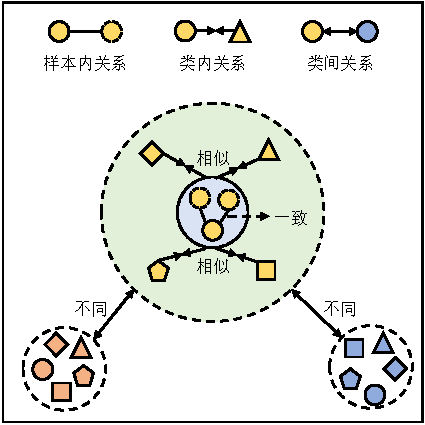
\includegraphics[width=0.6\columnwidth]{figures/MGSRCL/SampleRelation.pdf}
% \captionsetup{justification=justified,singlelinecheck=false}
\bicaption[样本关系示意图]{样本关系示意图。在该图中,不同形状与颜色分别代表不同样本与类别。同一样本的不同变换由相同的颜色和形状表示。样本关系包括三种类型:样本内关系、类内关系和类间关系。本章所提方法约束同一样本不同变换版本在语义内容上保持一致,同类样本保持相似,非同类样本保持不同。}[Illustration of sample relations]{Illustration of sample relations. In this figure, different shapes and different colors represent different samples and different classes, respectively. Different transformations of the same sample are represented by the same color and shape. The sample relations contain three types: intra-sample relation, intra-class relation and inter-class relation. The approach proposed in this chapter enforces different transformations to be consistent in semantic content, homogenous samples to be similar, and inhomogeneous samples to be different.}
\label{figure3: sample relation}
\end{figure}

\subsection[\hspace{-2pt}方法概述]{{\heiti\zihao{4} \hspace{-8pt}方法概述}}\label{section3: 方法概述}

为了解决上述问题,本文重新审视了多种样本关系,并提出了一个针对少样本分类的多粒度样本关系对比学习(Multi-Grained Sample Relation Contrastive Learning, 简称MGSRCL)方法。MGSRCL将样本关系分为三种不同粒度的类型:同一样本不同变换版本的样本内关系(intra-sample relation),同类样本的类内关系(intra-class relation),以及不同类样本的类间关系(inter-class relation),这三种样本关系揭示了数据在不同层次的内在结构和差异,如图\ref{figure3: sample relation}所示。

针对这三种不同粒度的样本关系,MGSRCL提出了两个模块对其进行约束。首先对于同一样本不同变换间的样本内关系,本文通过变换一致性学习(Transformation Consistency Learning,简称TCL)策略进行约束。这一策略的灵感来源于这样一个认识:同一样本在不同但轻微的变换下应保持其本质的语义不变性。TCL通过对齐样本及其变换版本的预测标签分布来确保其在标签输出上的一致性,从而保证样本和其不同变换版本在特征空间保持高度的语义一致性。第二种样本关系是同类样本的类内关系,由于同类样本的语义内容不像同一样本不同变换那样高度一致,忽视同类样本之间的语义差异并将它们映射到特征空间中的同一位置会因为简化了模型的学习过程而导致模型崩塌。因此,本文采用类对比学习(Class Contrastive Learning,简称CCL)来以一种相对的形式约束这种样本关系以及第三种样本关系,即不同类样本的类间关系。CCL不追求同类样本在特征空间中的绝对一致性,而着重于以一种相对距离的方式在特征空间中增强同类样本间的内聚程度,同时增大不同类别间的分离程度,从而提高了模型对不同类别样本的区分能力。

以验证本章方法的有效性,本章在四个基准数据集上进行了广泛的实验,包括三个普通少样本分类数据集:miniImageNet\cite{vinyals2016matching}、tieredImageNet\cite{ren2018meta}、CIFAR-FS\cite{bertinetto2019meta},以及一个细粒度少样本分类数据集:CUB-200-2011\cite{wah2011caltech}。实验结果表明,本章方法取得了优异的结果,并且可以作为预训练模型提升其他两阶段少样本分类方法的性能。


\section[\hspace{-2pt}基于多粒度样本关系对比学习的少样本特征学习算法]{{\heiti\zihao{-3} \hspace{-8pt}基于多粒度样本关系对比学习的少样本特征学习算法}}\label{section3: 基于多粒度样本关系对比学习的少样本特征学习算法}

在本节中,首先对少样本分类任务及其符号定义进行介绍;然后对所提出的基于多粒度样本关系对比学习的少样本特征学习模型进行简要介绍;接下来详细介绍了所提模型的各个模块及其损失优化;最后介绍了模型总体优化目标以及模型推理过程。

\subsection[\hspace{-2pt}符号定义]{{\heiti\zihao{4} \hspace{-8pt}符号定义}}\label{section3: 符号定义}

在本章中,少样本分类任务的基类数据集和新类数据集分别表示为:
\begin{equation}
\begin{aligned}
  &\mathcal{D}_{base} = \{(x, y)|x \in X^{base}, y \in Y^{base}\}, \\
  &\mathcal{D}_{novel} = \{(x, y)|x \in X^{novel}, y \in Y^{novel}\}.
\end{aligned}
\end{equation}
其中,$\mathcal{D}_{base}$所包含的类别$\mathcal{C}_{base}$和$\mathcal{D}_{novel}$所包含的类别$\mathcal{C}_{novel}$不相交。另外,$x$、$y$分别表示样本图像和样本标签;$X^{base}$、$Y^{base}$和$X^{novel}$、$Y^{novel}$分别表示基类数据和新类数据的样本图像集合和标签集合。

$\mathcal{D}_{base}$用于在预训练阶段训练一个具有良好泛化性能的模型,$\mathcal{D}_{novel}$用于测试过程采样大量\emph{N}-way \emph{K}-shot少样本分类任务并计算平均准确率来评估模型性能。每个少样本分类任务$\mathcal{T}$包括一个支持集$\mathcal{S}_\mathcal{T}$和一个查询集$\mathcal{Q}_\mathcal{T}$,
\begin{equation}
  \mathcal{T} = \{\mathcal{S}_\mathcal{T}, \mathcal{Q}_\mathcal{T}\}.
\end{equation}
其中,$\mathcal{S}_\mathcal{T}$包含来自\emph{N}个类别的\emph{N} $\times$ \emph{K}个标注样本,而$\mathcal{Q}_\mathcal{T}$包含来自相同\emph{N}个类别的\emph{N} $\times$ \emph{Q}个样本,并且$\mathcal{S}_\mathcal{T}$和$\mathcal{Q}_\mathcal{T}$中的样本是没有交集的。在测试阶段,针对每个采样的少样本分类任务使用$\mathcal{S}_\mathcal{T}$重新训练一个分类器,使用$\mathcal{Q}_\mathcal{T}$来评估分类器性能。

\begin{figure}[h!]
\centering
\captionsetup{font={small, stretch=1.312}}
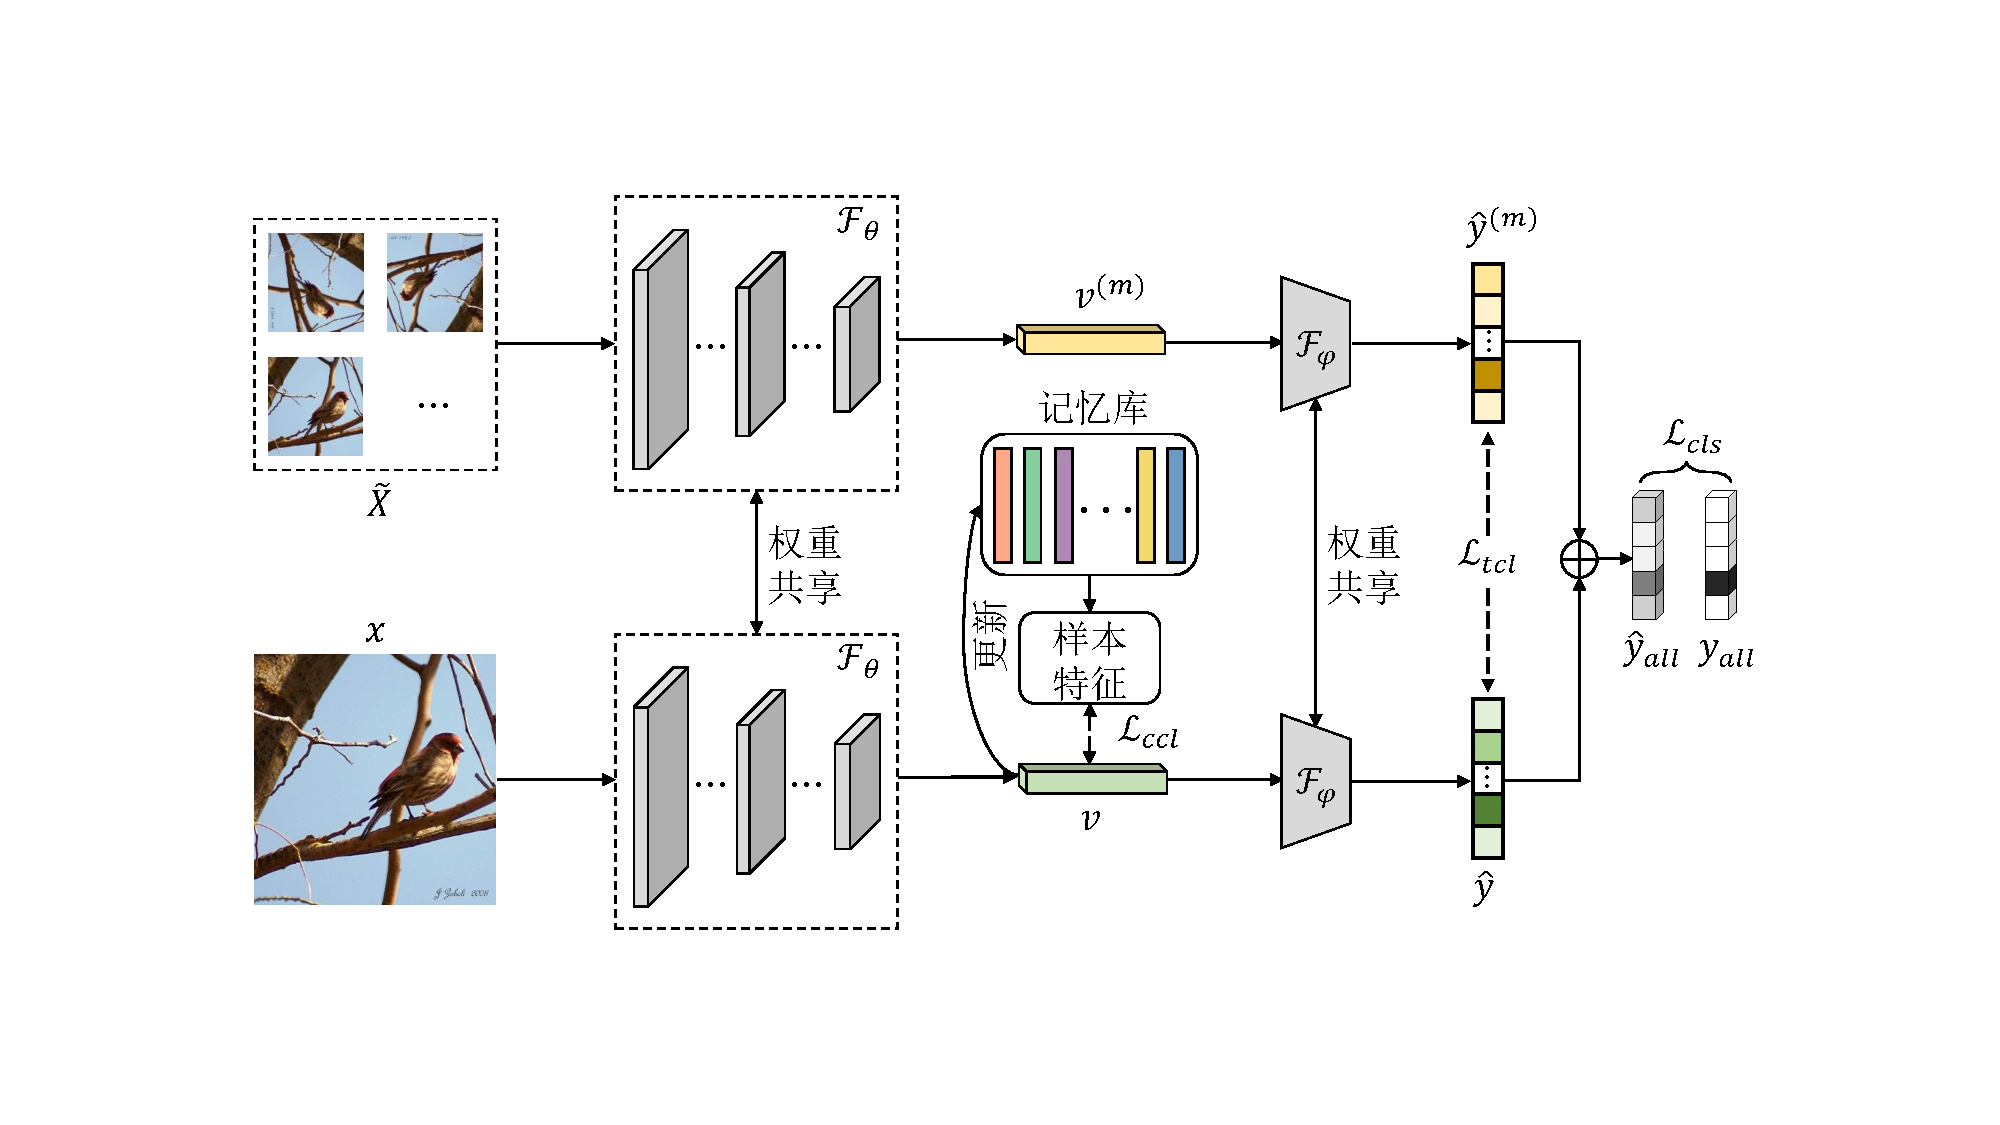
\includegraphics[width=1.0\columnwidth]{figures/MGSRCL/model.pdf}
% \captionsetup{justification=justified,singlelinecheck=false}
\bicaption[多粒度样本关系对比学习模型示意图]{多粒度样本关系对比学习模型(MGSRCL)示意图。它包含一个特征提取网络$\mathcal{F}_{\theta}$和一个分类器$\mathcal{F}_{\varphi}$。在此图中,$v$和$v^{(m)}$代表原始图像$x$及其第$m$个变换版本$x^{(m)}$的特征,其中$x^{(m)} \in \widehat{X}$。$\bigoplus$是一个连接操作,用于对原始图像的预测输出$\widehat{y}$与$M$个变换的预测输出${\widehat{y}^{(1)}, ..., \widehat{y}^{(m)}, ..., \widehat{y}^{(M)}}$进行连接。记忆库(Memory Bank)用于存储特征。$\mathcal{L}_{cls}$,$\mathcal{L}_{tcl}$和$\mathcal{L}_{ccl}$分别是分类损失、变换一致性学习(TCL)损失和类对比学习(CCL)损失。为了便于阅读,此图中没有展示自监督模块。}[Illustration of Multi-Grained Sample Relation Contrastive Learning (MGSRCL) model]{Illustration of Multi-Grained Sample Relation Contrastive Learning (MGSRCL) model. It contains a feature extraction network $\mathcal{F}_{\theta}$ and a classifier $\mathcal{F}_{\varphi}$. In this figure, $v$ and $v^{(m)}$ represent the features of the original image $x$ and its $m$-th transformed version $x^{(m)}$,where $x^{(m)} \in \widehat{X}$. $\bigoplus$ is a concatenation operator for the predicted output $\widehat{y}$ of the original image and the predicted outputs $\{\widehat{y}^{(1)}, ..., \widehat{y}^{(m)}, ..., \widehat{y}^{(M)}$\} of $M$ transformations. Memory bank is used to store the features. $\mathcal{L}_{cls}$, $\mathcal{L}_{tcl}$, and $\mathcal{L}_{ccl}$ are the classification loss, transformation consistency learning (TCL) loss, and class contrastive learning (CCL) loss, respectively. For the sake of legibility, the self-supervised module is not shown in this image.}
\label{figure3: model}
\end{figure}

\subsection[\hspace{-2pt}整体框架]{{\heiti\zihao{4} \hspace{-8pt}整体框架}}\label{section3: 整体框架}

本章重新审视了对比学习中的样本关系,并根据样本关系粒度的不同将其划分为三种类型:同一样本在不同变换下的样本内关系(intra-sample relation)、同类样本的类内关系(intra-class relation),以及不同类样本的类间关系(inter-class relation)。基于此,本章提出了一种新颖的多粒度样本关系对比学习方法(Multi-Grained Sample Relation Contrastive Learning,简称MGSRCL),通过对少样本分类中不同粒度的样本关系进行建模从而获得了一个强大的特征提取网络。如图\ref{figure3: model}所示,MGSRCL模型包含三个主要部分:基础特征学习网络(Base Feature Learning Network,简称Base)、变换一致性学习(Transformation Consistency Learning,简称TCL)模块和类对比学习(Class Contrastive Learning,简称CCL)模块。具体而言,基础特征学习网络是通过一般图像分类任务训练的神经网络。TCL模块旨在确保同一样本的不同变换版本具有一致的语义内容。而CCL则用于确保同类样本具有相似的语义内容,以及非同类样本具有不同的语义内容。接下来,本节将对MGSRCL方法的每个部分进行更为详细的阐述。

\subsection[\hspace{-2pt}基础特征学习网络]{{\heiti\zihao{4} \hspace{-8pt}基础特征学习网络}}\label{section3: 基础特征学习网络}

如图\ref{figure3: model}所示,特征提取网络,表示为带有参数$\theta$的$\mathcal{F}_{\theta}$,被用于提取图像特征。设$(x, y)\in \mathcal{D}_{base}$表示从$\mathcal{D}_{base}$中采样的图像及其对应的标签。图像$x$的特征向量$v$可以通过$\mathcal{F}_{\theta}$获得:$v=\mathcal{F}_{\theta}(x)$。然后,使用参数为$\varphi$的分类器$\mathcal{F}_{\varphi}$,将特征向量$v$投影到标签空间,以获得预测的置信度分数$p$:$p=\mathcal{F}_{\varphi}(v)$。最后,通过在$p$上应用Softmax函数,可以得到预测概率输出$\widehat{y}$:$\widehat{y}=\text{Softmax}(p)$。基础特征学习网络的参数$\theta$和$\varphi$通过最小化整个基类数据集$\mathcal{D}_{base}$上的分类损失$\mathcal{L}_{cls}$来进行优化,其可以表示为以下公式,
\begin{equation}
\label{equation3:3.2}
  \mathcal{L}_{cls} = - \frac{1}{|\mathcal{D}_{base}|}\sum_{\{x,y\}\in \mathcal{D}_{base}}y\log\widehat{y}.
\end{equation}

为了防止在训练集上过拟合,许多方法\cite{IER, PAL, SSLforFSL}引入了变换样本参与训练,并使用自监督学习技术预测在训练过程中对图像执行了哪种变换以增强网络的特征提取能力。遵循这些方法,本文也添加了一个由多层感知机(Multilayer Perceptron,简称MLP)构成的自监督(Self-Supervised,简称SS)模块。设$\widetilde{X}=\{\widetilde{x}^{(1)}, ..., \widetilde{x}^{(M)}\}$为一张图像的变换版本集合,其中$M$表示变换样本的总数,$\widetilde{x}^{(m)}$表示图像的第$m$个变换版本。$\widetilde{X}$可以通过在图像上应用一系列变换(如裁剪、调整大小、旋转等数据增强操作)获得。变换后的图像$\widetilde{X}$和原始图像$x$同时输入模型,用于分类和自监督任务。自监督任务的目标是识别图像进行了哪种变换,其损失$\mathcal{L}_{ss}$表示为以下公式,
\begin{equation}
\label{equation3:3.3}
  \mathcal{L}_{ss} = - \frac{1}{|\mathcal{D}_{base}|}\frac{1}{M+1}\sum_{x \in \mathcal{D}_{base}}\sum_{m=0}^{M}s^{(m)}\log\widehat{s}^{(m)},
\end{equation}
其中$\widehat{s}^{(m)}$和$s^{(m)}$分别表示自监督任务中第$m$个变换版本的预测概率输出和真实标签。$s^{(0)}$是原始图像$x$的自监督标签。此外,增加了变换样本之后的分类损失可以重新定义为以下公式,
\begin{equation}
\label{equation3:3.4}
  \mathcal{L}_{cls} = - \frac{1}{|\mathcal{D}_{base}|}\frac{1}{M+1}\sum_{x \in \mathcal{D}_{base}}\sum_{m=0}^{M}y^{(m)}\log\widehat{y}^{(m)},
\end{equation}
$\widehat{y}^{(m)}$表示分类任务中的预测概率输出,$y^{(m)}$表示分类任务的真实标签。

最后,基础特征学习网络的损失$\mathcal{L}_{base}$可以写为分类损失$\mathcal{L}_{cls}$和自监督损失$\mathcal{L}_{ss}$之和,
\begin{equation}
\label{equation3:3.5}
  \mathcal{L}_{base} = \mathcal{L}_{cls} + \mathcal{L}_{ss}.
\end{equation}

\subsection[\hspace{-2pt}多粒度样本关系对比学习算法]{{\heiti\zihao{4} \hspace{-8pt}多粒度样本关系对比学习算法}}\label{section3: 多粒度样本关系对比学习算法}

\textbf{(1)变换一致性学习}

一个样本图像与其变换版本包含完全相同的对象和背景,仅因为进行了数据增强而使得图像在旋转角度、明暗、颜色等方面发生变化,但其内在的类别属性和语义内容应保持不变。为了实现这一目标,本文设计了一个变换一致性学习(Transformation Consistency Learning,简称TCL)模块,以约束同一样本不同变换版本的样本内关系。TCL模块通过约束一个样本和其变换版本的预测输出相同来确保它们具有一致的语义内容。这是因为预测输出反映了样本在每个类别中的预测概率,这些概率不仅表示了模型对于样本属于各个类别的置信度,而且深入地揭示了样本的本质属性——语义内容。

本章方法将一个样本与其变换版本同时输入网络,并在预测标签输出层面计算它们的TCL损失。这里,本文使用Jensen-Shannon散度\cite{JS1, JS2}作为TCL损失,它能够衡量两个概率分布的差异,通过最小化两个预测标签的输出,可以使其概率分布一致,从而达到使样本和其变换版本具有一致语义内容的目的。TCL损失可以写为以下公式,
\begin{equation}
\label{equation3:3.6}
  \mathcal{L}_{tcl} = \frac{1}{|\mathcal{D}_{base}|}\sum_{x \in \mathcal{D}_{base}}\frac{1}{M}\sum_{m=1}^{M}JS(\widehat{y}_{\tau_1}, \widehat{y}_{\tau_1}^{(m)}),
\end{equation}
其中$\widehat{y}_{\tau_1}$和$\widehat{y}_{\tau_1}^{(m)}$分别是原始图像和第$m$个变换图像的平滑标签输出。它们通过以下公式获得,
\begin{equation}
\label{equation3:3.7}
  \widehat{y}_{\tau_1} = \text{Softmax}(p/\tau_1),
\end{equation}
此公式中$p = \mathcal{F}_{\varphi}(\mathcal{F}_{\theta}(x))$,$\tau_1$是一个温度参数,本文在实验中将其设置为$4.0$。使用平滑标签输出的原因在于不同变换的输出不仅需要在最大预测概率的类别上保持一致,而且需要在所有其他类别上也保持一致,以确保它们具有完全相同的语义内容,而平滑标签输出可以提供更多关于概率分布差异的信息。

\textbf{(2)类对比学习}

同类样本虽然图像内包含了同一个类别的物体,但物体及其背景与同一图像不同变换版本相比差异性较大,因此其预测概率输出之间差异也会较大。如果强行将其预测输出进行对齐,可能会使得网络为了学习此种强关系而导致模型崩塌。但在另一方面,同类样本间距离比不同类样本间距离更近是毋庸置疑的。因此,本文采用类对比学习(Class Contrastive Learning,简称CCL)以一种相对距离的形式约束同类样本的类内关系和不同类样本的类间关系。CCL模块通过最大化同类样本特征的相似性,同时最小化不同类样本特征的相似性来在特征空间拉近同类样本,推远不同类样本。

与之前对比学习不同,CCL模块为了将样本和其他每个不同类间的距离推远,对于每张图像都需要该图像的一个同类样本以及其他每个类别的不同类样本(之前对比学习通常随机采样,这使得每个批次计算损失时不同类样本可能仅来自部分不同类别)。为了实现这一目标并加快训练速度,本文使用了一个记忆库(Memory Bank)来存储和从中采样图像特征,记忆库存储了所有图像的特征。在一个批次中,CCL模块从记忆库中为每类图像随机采样一个样本的特征。CCL损失可以定义为,
\begin{equation}
\label{equation3:3.8}
  \mathcal{L}_{ccl} = \frac{1}{|\mathcal{D}_{base}|}\sum_{x \in \mathcal{D}_{base}}-\log \frac{\text{exp}(\frac{cos(v, v^\prime)}{\tau_2})}{\sum_{i=1}^{|\mathcal{C}_{base}|}{\text{exp}(\frac{cos(v, v_i)}{\tau_2})}},
\end{equation}
其中$|\mathcal{C}_{base}|$和$|\mathcal{D}_{base}|$表示基类的类别数量和样本数量,$v$和$v^\prime$分别是某个样本及其同类样本的特征,$v_i$代表来自第$i$类的样本的特征。这里$v^\prime$和$v_i$是从记忆库中采样的。$cos(\cdot)$是余弦相似度,$\text{exp}(\cdot)$为以e为底的指数函数。而$\tau_2$是一个温度参数,本文按照\cite{SimCLR, SupCon}的实验设置将其设为$0.1$。此外,记忆库的更新方式为,
\begin{equation}
\label{equation3:3.9}
  v_{k} = r\times v_k + (1 - r)\times v_q,
\end{equation}
$v_q$和$v_k$分别代表在当前小批次中获得的图像特征以及在记忆库中存储的相同图像的特征,$r$用于调整记忆库的更新速度,按照IER方法\cite{IER}的实验,本文将其设置为$0.99$。在训练阶段,记忆库每一轮训练过程都会完全更新一遍。

\subsection[\hspace{-2pt}模型优化]{{\heiti\zihao{4} \hspace{-8pt}模型优化}}\label{section3: 模型优化}
结合公式\ref{equation3:3.5}、\ref{equation3:3.6}和\ref{equation3:3.8},本章提出的MGSRCL模型总体损失函数可以表示为以下公式,
\begin{equation}
\label{equation3:3.10}
  \mathcal{L}_{total} = \mathcal{L}_{base} + \alpha \cdot \mathcal{L}_{tcl} + \beta \cdot \mathcal{L}_{ccl},
\end{equation}
其中$\alpha$和$\beta$是用于平衡不同损失的超参数,分别表示TCL模块和CCL模块的损失权重。

MGSRCL模型通过在整个基类数据集上最小化上述损失函数对模型参数进行联合优化。通过建模多个粒度的样本关系,可以有效地增强模型的特征提取能力和泛化能力,帮助模型捕获更具判别性的特征,从而提高模型在新类$\mathcal{D}_{novel}$上的分类性能。

\subsection[\hspace{-2pt}模型推理]{{\heiti\zihao{4} \hspace{-8pt}模型推理}}\label{section3: 模型推理}
模型在基类数据集$\mathcal{D}_{base}$训练完成之后,在测试阶段,将会冻结MGSRCL模型特征提取网络的所有参数,并通过解决来自新类$\mathcal{D}_{novel}$的大量少样本分类任务来评估模型性能。在每个任务$\mathcal{T}$的推理过程中,本文使用特征提取网络$\mathcal{F}_{\theta}$来获得支持集$\mathcal{S}_\mathcal{T}$和查询集$\mathcal{Q}_\mathcal{T}$的图像特征。然后,本文使用$\mathcal{S}_\mathcal{T}$的样本特征训练一个逻辑回归分类器$LC$,并对$\mathcal{Q}_\mathcal{T}$中的样本进行分类,最后将在多个少样本分类任务上的准确率平均值作为模型的评价指标。MGSRCL模型的推理过程如图\ref{figure3: 推理过程}所示。

\begin{figure}[h]
\centering
\captionsetup{font={small, stretch=1.312}}
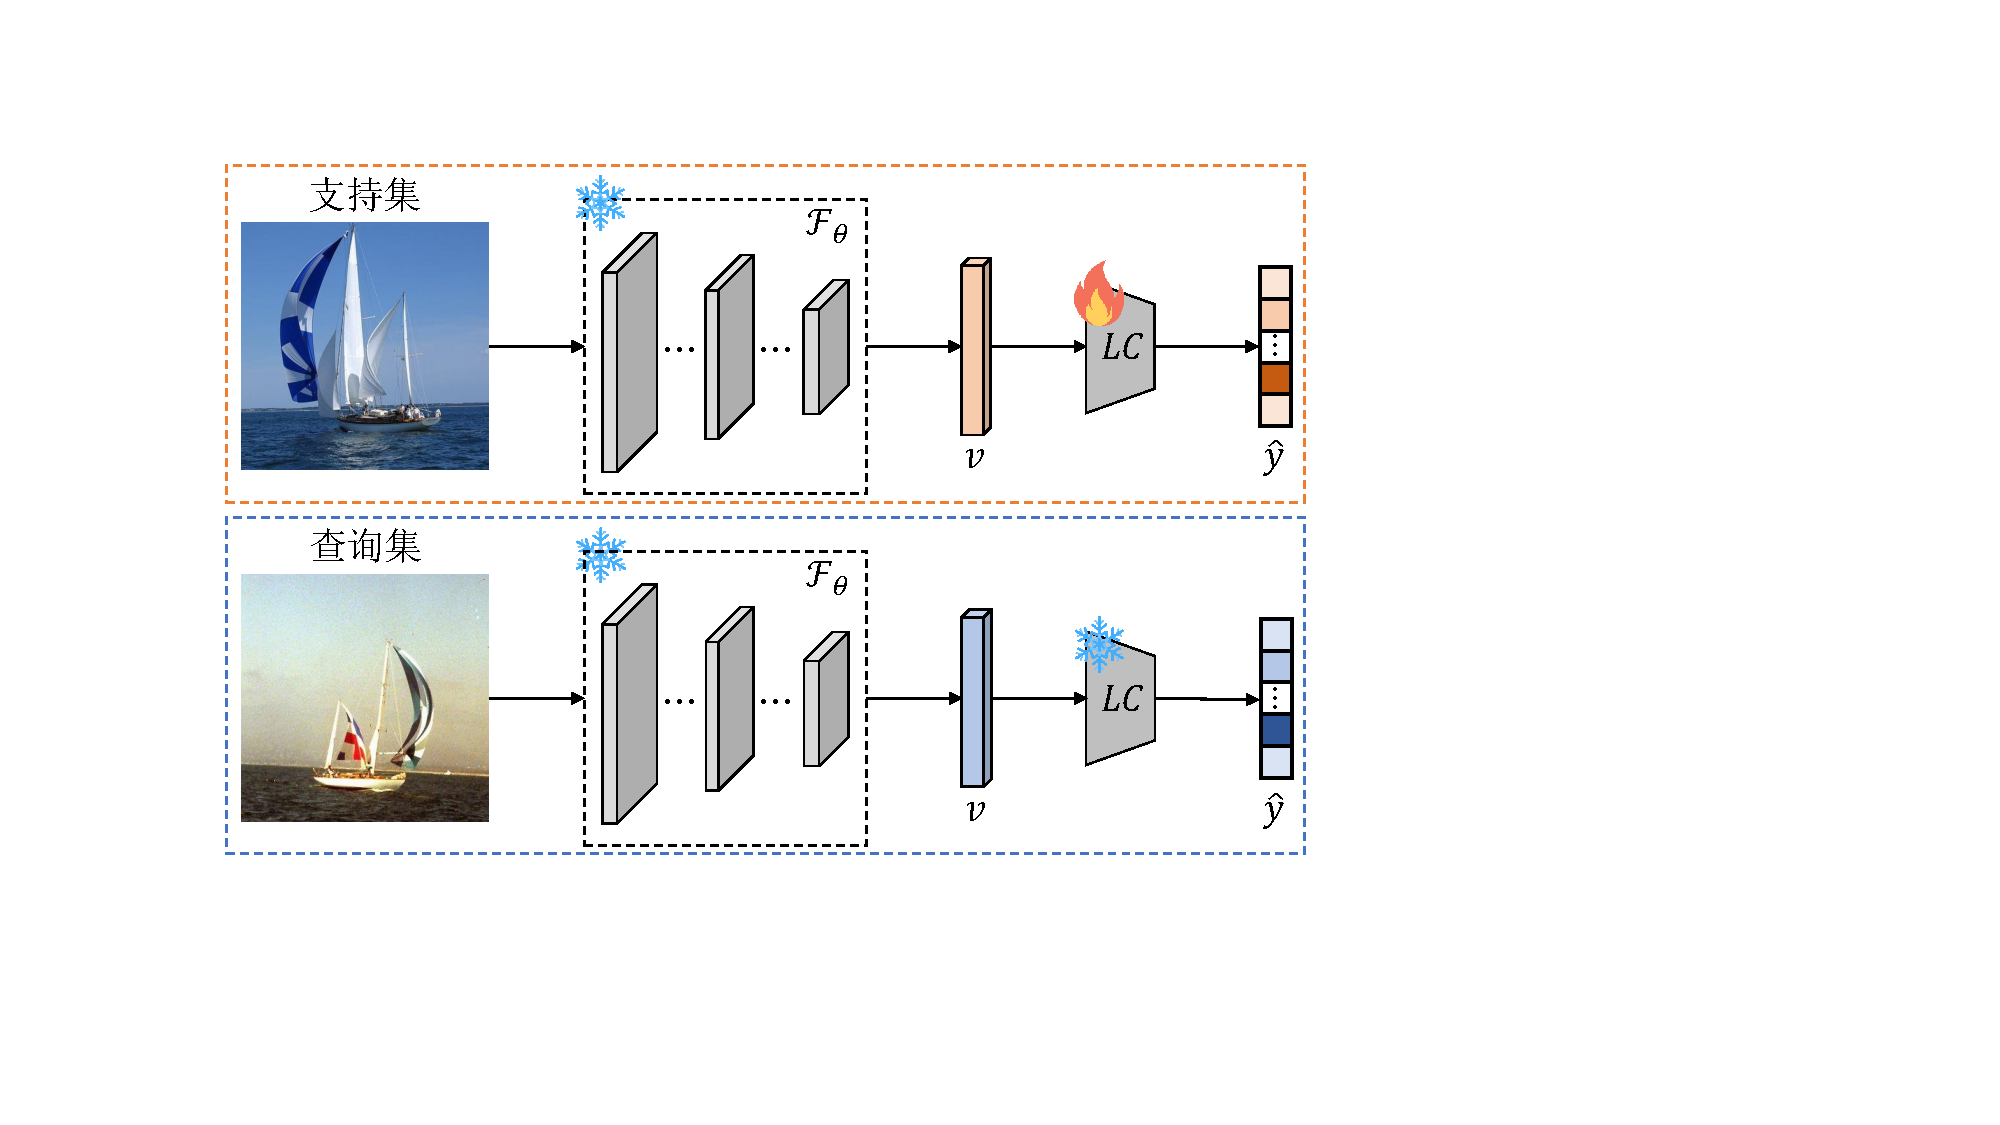
\includegraphics[width=0.8\columnwidth]{figures/MGSRCL/推理过程.pdf}
% \captionsetup{justification=justified,singlelinecheck=false}
\bicaption[MGSRCL模型推理过程示意图]{MGSRCL模型推理过程示意图。推理过程中,使用冻结参数的特征提取网络$\mathcal{F}_{\theta}$提取支持集与查询集的图像特征。其中,支持集特征被用来训练一个逻辑回归分类器$LC$,查询集特征则是用来测试分类器性能。}[Illustration of MGSRCL model inference process]{Illustration of MGSRCL model inference process. During the inference process, the feature extraction network $\mathcal{F}_{\theta}$ with frozen parameters is used to extract image features from both support set and query set. Herein, the support set features are utilized to train a logistic regression classifier $LC$, while the query set features are used to assess the classifier's performance.}
\vspace{-10pt}
\label{figure3: 推理过程}
\end{figure}

\section[\hspace{-2pt}实验设置及结果分析]{{\heiti\zihao{-3} \hspace{-8pt}实验设置及结果分析}}\label{section3: 实验设置及结果分析}
在本节中,首先介绍了本章方法的实验设置,包括数据集设置、网络结构、优化设置、数据增强方式,然后分析了基于多粒度样本关系对比学习的少样本特征学习算法实验结果,接下来对模型的多个模块以及超参数进行了消融实验和分析,最后对模型所提取特征进行了可视化分析。

\subsection[\hspace{-2pt}实验设置]{{\heiti\zihao{4} \hspace{-8pt}实验设置}}\label{section3: 实验设置}

\textbf{(1)实验数据集介绍}

本文在四个常用的少样本分类基准数据集上进行了实验,其中包括三个普通少样本分类数据集:miniImageNet \cite{vinyals2016matching}、tieredImageNet \cite{ren2018meta}、CIFAR-FS \cite{bertinetto2019meta},以及一个细粒度数据集:CUB-200-2011(CUB)\cite{wah2011caltech}。对于所有数据集,本文保持了与其他工作\cite{RFS, RENet, IER}相同的划分准则。在实验中,对于miniImageNet、tieredImageNet和CUB,图像大小为84$\times$84,而对于CIFAR-FS,图像大小为32$\times$32。

\textbf{(2)网络结构}

遵循先前的研究工作\cite{RFS, DeepEMD, IER},本文采用了ResNet-12作为特征提取网络。变换一致性学习(TCL)在标签输出上进行,而类对比学习(CCL)在经过全局池化层后的特征上进行,这些技术不需要额外的网络层。此外,本文添加了一个自监督学习模块,该模块是一个由两个全连接层、一个批归一化层和一个激活函数组成的多层感知机。

\textbf{(3)优化设置}

在所有实验中,本文使用了具有0.9动量和$5e^{-4}$权重衰减的随机梯度下降(Stochastic Gradient Descent,简称SGD)优化器。初始学习率设定为0.05,随后在特定轮次以0.1的倍数衰减。对于tieredImageNet,总共训练了60个轮次,学习率分别在第30、40和50轮次后衰减。对于其他数据集,训练了80个轮次,学习率在第60和70轮次后衰减。关于超参数,本文对所有数据集设置为以下值:$\alpha=1.0$,$\beta=0.1$,$\tau_1=4.0$,$\tau_2=0.1$。

\textbf{(4)数据增强}

为了缓解过拟合问题并进行MGSRCL模型中的变换一致性学习(TCL),本文在训练特征提取网络时添加了一些数据增强样本。数据增强包括三种长宽比例不同的裁剪缩放变换、三种旋转变换(分别为90°、180°和270°)、一种随机擦除、一种图像灰度化和一种Sobel边缘检测。在训练过程中,这些数据增强样本与原始样本一同作为模型的输入。

\subsection[\hspace{-2pt}基准数据集实验结果]{{\heiti\zihao{4} \hspace{-8pt}基准数据集实验结果}}\label{section3: 基准数据集实验结果}

为了评估方法的有效性,本文在四个数据集上进行了广泛的实验。模型评估过程中,对5-way 1-shot以及5-way 5-shot分别采样2000个任务并计算平均分类准确率作为最终实验结果。表\ref{table3: mini}、\ref{table3: tiered}、\ref{table3: CIFAR-FS}和\ref{table3: CUB}分别展示了miniImageNet、tieredImageNet、CIFAR-FS和CUB数据集上一些现有少样本分类方法和本文方法的实验结果。此外,本文还将所提模型作为预训练网络结合到三个两阶段少样本分类算法中,并与原方法性能进行对比以进一步验证本文所获得特征提取网络的有效性。另外,部分直推式少样本分类方法\cite{cui2021parameterless, qi2021transductive}虽然取得了更好的实验结果,但由于其训练过程模型可以使用测试数据,与本文设置不同,因此不与其进行对比(第四章中相同)。


\textbf{(1)普通少样本分类}

如表\ref{table3: mini}和\ref{table3: tiered}所示,本文方法MGSRCL在miniImageNet和tieredImageNet数据集上与其他方法相比取得了出色的性能。具体而言,MGSRCL在miniImageNet上的1-shot和5-shot任务中分别达到了69.57\%和84.41\%的准确率,在tieredImageNet上分别达到了72.98\%和86.23\%的准确率。特别是在5-way 1-shot任务中,MGSRCL达到了最优实验结果,在两个数据集上分别比次优结果高0.20\%和0.30\%。在CIFAR-FS数据集上,MGSRCL在1-shot和5-shot少样本分类任务中分别达到了78.54\%和88.64\%的准确率,在1-shot任务上比次优的PAL方法高1.44\%,如表\ref{table3: CIFAR-FS}所示。值得注意的是,与采用知识蒸馏技术的RFS\cite{RFS}、PAL\cite{PAL}和SCL\cite{Spatial},以及使用元学习方法的DeepEMD\cite{DeepEMD}和ESPT\cite{ESPT}不同,MGSRCL无需进行第二次训练或元学习微调阶段。本文方法使得预训练模型能够达到与最先进方法相媲美甚至超越的性能,这证明了所提方法能够增强模型的特征提取能力和泛化能力,从而使得所提取到的新类特征具有更好的判别性。

{\small    % 设置表格字体为5号
\setstretch{1.245}        % 设置具有指定弹力的橡皮长度(原行宽的1.2倍)
\captionsetup{font={small, stretch=1.512}}
\begin{xltabular}{\textwidth}{lCCC}
\bilingualcaption{MGSRCL在miniImageNet数据集上的分类准确率(\%)}{MGSRCL在miniImageNet数据集上的分类准确率(\%)。最优结果用粗体表示,带有“\dag”标记的方法表示结果是使用作者提供代码所实现。}{Classification accuracy (\%) of MGSRCL on miniImageNet. The best results are shown in bold, and methods with the ``\dag'' indicate that the result was implemented using author-supplied code.}
\label{table3: mini} \\
\toprule
方法 & 特征提取网络 & 5-way 1-shot & 5-way 5-shot \\
\midrule
\endfirsthead

\multicolumn{4}{c}{\tablename \thetable{} (续)} \\ % 第一行标题
\multicolumn{4}{c}{Table \thetable{} (continued)} \\ % 第二行标题

\toprule
方法 & 特征提取网络 & 5-way 1-shot & 5-way 5-shot \\
\midrule
\endhead

% \midrule \multicolumn{3}{r}{{接下页}} \\ 
\bottomrule
\endfoot

\bottomrule
\endlastfoot

% 添加你的内容
MAML \cite{MAML} & 32-32-32-32 & 48.70 $\pm$ 1.84 & 63.11 $\pm$ 0.92 \\
ProtoNet \cite{ProtoNet} & 64-64-64-64 & $ 49.42 \pm 0.78 $ & 68.20 $\pm$ 0.66 \\
DeepEMD \cite{DeepEMD} & ResNet-12 & 65.91 $\pm$ 0.82 & 82.41 $\pm$ 0.56 \\
RFS-distill \cite{RFS} & ResNet-12 & 64.82 $\pm$ 0.60 & 82.14 $\pm$ 0.43 \\
AssoAlign \cite{AssoAlign} & ResNet-18 & 59.88 $\pm$ 0.67 & 80.35 $\pm$ 0.73 \\
GIFSL \cite{GIFSL} & ResNet-12 & 65.47 $\pm$ 0.63 & 82.75 $\pm$ 0.42 \\
MELR \cite{MELR} & ResNet-12 & 67.40 $\pm$ 0.43 & 83.40 $\pm$ 0.28\\
IEPT \cite{IEPT} & ResNet-12 & 67.05 $\pm$ 0.44 & 82.90 $\pm$ 0.30 \\
IER \cite{IER} & ResNet-12 & 66.82 $\pm$ 0.80 & 84.35 $\pm$ 0.51 \\
RENet \cite{RENet} & ResNet-12 & 67.60 $\pm$ 0.44 & 82.58 $\pm$ 0.30 \\
PAL \cite{PAL} & ResNet-12 & 69.37 $\pm$ 0.64 & 84.40 $\pm$ 0.44 \\
HandCrafted \cite{HandCrafted} & ResNet-12 & 67.14 $\pm$ 0.76 & 83.11 $\pm$ 0.69 \\
PDA \cite{PDA} & ResNet-12 & 65.75 $\pm$ 0.43 & 83.37 $\pm$ 0.30 \\
SCL-distill \cite{Spatial} & ResNet-12 & 67.40 $\pm$ 0.76 & 83.19 $\pm$ 0.54 \\
HGNN \cite{HGNN} & ResNet-12 & 67.02 $\pm$ 0.20 & 83.00 $\pm$ 0.13 \\
APP2S \cite{APP2S} & ResNet-18 & 64.82 $\pm$ 0.12 & 81.31 $\pm$ 0.22 \\
DGAP \cite{DGAP} & ResNet-12 & 61.35 $\pm$ 0.62 & 78.85 $\pm$ 0.46 \\
ESPT \cite{ESPT} & ResNet-12 & 68.36 $\pm$ 0.19 & 84.11 $\pm$ 0.12 \\
Meta-HP \cite{Meta-HP} & ResNet-12 & 62.49 $\pm$ 0.80 & 77.12 $\pm$ 0.62 \\
SAPENet \cite{SAPENet} & ResNet-12 & 66.41 $\pm$ 0.20 & 82.76 $\pm$ 0.14 \\
FEAT+DFR \cite{DFR} & ResNet-12 & 67.74 $\pm$ 0.86 & 82.49 $\pm$ 0.57 \\
DiffKendall \cite{DiffKendall} & ResNet-12 & 65.56 $\pm$ 0.43 & 80.79 $\pm$ 0.31 \\
\midrule
FEAT \cite{FEAT} & ResNet-12 & 66.78 $\pm$ 0.20 & 82.05 $\pm$ 0.14 \\
\textbf{MGSRCL + FEAT} & ResNet-12 & 69.27 $\pm$ 0.21 & 83.59 $\pm$ 0.13 \\
\midrule
Meta-Baseline\dag \cite{MetaBaseline} & ResNet-12 & 63.38 $\pm$ 0.23 & 79.48 $\pm$ 0.16 \\
\textbf{MGSRCL + Meta-Baseline} & ResNet-12 & 69.01 $\pm$ 0.23 & 83.94 $\pm$ 0.15 \\
\midrule
STVAE \cite{STVAE} & ResNet-12 & 63.62 $\pm$ 0.80 & 80.68 $\pm$ 0.48 \\
\textbf{MGSRCL + STVAE} & ResNet-12 & 67.29 $\pm$ 0.89 & 82.62 $\pm$ 0.58 \\
\midrule
\textbf{MGSRCL} & ResNet-12 & \textbf{69.57 $\pm$ 0.45} & \textbf{84.41 $\pm$ 0.30} \\
\end{xltabular}}


{
\small    % 设置表格字体为5号
\setstretch{1.245}        % 设置具有指定弹力的橡皮长度(原行宽的1.2倍)
\captionsetup{font={small, stretch=1.512}}
\begin{xltabular}{\textwidth}{lCCC}
\bilingualcaption{MGSRCL在tieredImageNet数据集上的分类准确率(\%)}{MGSRCL在tieredImageNet数据集上的分类准确率(\%)。最优结果用粗体表示,带有“\dag”标记的方法表示结果是使用作者提供代码所实现。}{Classification accuracy (\%) of MGSRCL on tieredImageNet. The best results are shown in bold, and methods with the ``\dag'' indicate that the result was implemented using author-supplied code.}
\label{table3: tiered} \\
\toprule
方法 & 特征提取网络 & 5-way 1-shot & 5-way 5-shot \\
\midrule
\endfirsthead

\multicolumn{4}{c}{\tablename \thetable{} (续)} \\ % 第一行标题
\multicolumn{4}{c}{Table \thetable{} (continued)} \\ % 第二行标题

\toprule
方法 & 特征提取网络 & 5-way 1-shot & 5-way 5-shot \\
\midrule
\endhead

% \midrule \multicolumn{3}{r}{{接下页}} \\ 
\bottomrule
\endfoot

\bottomrule
\endlastfoot

% 添加你的内容
MAML \cite{MAML} & 32-32-32-32 & 51.67 $\pm$ 1.81 & 70.30 $\pm$ 1.75 \\
ProtoNet \cite{ProtoNet} & 64-64-64-64  & 53.31 $\pm$ 0.89 & 72.69 $\pm$ 0.74 \\
DeepEMD \cite{DeepEMD} & ResNet-12 & 71.16 $\pm$ 0.87 & 86.03 $\pm$ 0.58 \\
RFS-distill \cite{RFS} & ResNet-12 & 71.52 $\pm$ 0.69 & 86.03 $\pm$ 0.49 \\
AssoAlign \cite{AssoAlign} & ResNet-18 & 69.29 $\pm$ 0.56 & 85.97 $\pm$ 0.49 \\
GIFSL \cite{GIFSL} & ResNet-12 & 72.39 $\pm$ 0.66 & 86.91 $\pm$ 0.44 \\
MELR \cite{MELR} & ResNet-12 & 72.14 $\pm$ 0.51 & 87.01 $\pm$ 0.35 \\
IEPT \cite{IEPT} & ResNet-12 & 72.24 $\pm$ 0.50 & 86.73 $\pm$ 0.34 \\
IER \cite{IER} & ResNet-12 & 71.87 $\pm$ 0.89 & 86.82 $\pm$ 0.58 \\
RENet \cite{RENet} & ResNet-12 & 71.16 $\pm$ 0.51 & 85.28 $\pm$ 0.35 \\
PAL \cite{PAL} & ResNet-12 & 72.25 $\pm$ 0.72 & 86.95 $\pm$ 0.47 \\
PDA \cite{PDA} & ResNet-12 & 72.28 $\pm$ 0.49 & 86.70 $\pm$ 0.33 \\
SCL-distill \cite{Spatial} & ResNet-12 & 71.98 $\pm$ 0.91 & 86.19 $\pm$ 0.59 \\
HGNN \cite{HGNN} & ResNet-12 & 72.05 $\pm$ 0.23 & 86.49 $\pm$ 0.15 \\
APP2S \cite{APP2S} & ResNet-18 & 70.83 $\pm$ 0.15 & 84.15 $\pm$ 0.29 \\
DGAP \cite{DGAP} & ResNet-12 & 70.10 $\pm$ 0.67 & 84.99 $\pm$ 0.46 \\
ESPT \cite{ESPT} & ResNet-12 & 72.68 $\pm$ 0.22 & \textbf{87.49 $\pm$ 0.14} \\
Meta-HP \cite{Meta-HP} & ResNet-12 & 68.26 $\pm$ 0.72 & 82.91 $\pm$ 0.36 \\
SAPENet \cite{SAPENet} & ResNet-12 & 68.63 $\pm$ 0.23 & 84.30 $\pm$ 0.16 \\
FEAT+DFR \cite{DFR} & ResNet-12 & 71.31 $\pm$ 0.93 & 85.12 $\pm$ 0.64 \\
DiffKendall \cite{DiffKendall} & ResNet-12 & 70.76 $\pm$ 0.43 & 85.31 $\pm$ 0.34 \\
\midrule
FEAT \cite{FEAT} & ResNet-12 & 70.80 $\pm$ 0.23 & 84.79 $\pm$ 0.16 \\
\textbf{MGSRCL + FEAT} & ResNet-12 & 72.02 $\pm$ 0.23  & 86.19 $\pm$ 0.15 \\
\midrule
Meta-Baseline\dag \cite{MetaBaseline} & ResNet-12 & 68.74 $\pm$ 0.26 & 83.45 $\pm$ 0.18 \\
\textbf{MGSRCL + Meta-Baseline} & ResNet-12 & 69.79 $\pm$ 0.26 & 83.55 $\pm$ 0.18 \\
\midrule
STVAE\dag \cite{STVAE} & ResNet-12 & 68.32 $\pm$ 0.94 & 83.79 $\pm$ 0.66 \\
\textbf{MGSRCL + STVAE} & ResNet-12 & 72.03 $\pm$ 0.89 & 84.49 $\pm$ 0.66 \\
\midrule
\textbf{MGSRCL} & ResNet-12 & \textbf{72.98 $\pm$ 0.51} & 86.23 $\pm$ 0.34 \\
\end{xltabular}}

{
\small    % 设置表格字体为5号
\setstretch{1.245}        % 设置具有指定弹力的橡皮长度(原行宽的1.2倍)
\captionsetup{font={small, stretch=1.512}}
\begin{xltabular}{\textwidth}{lCCC}
\bilingualcaption{MGSRCL在CIFAR-FS数据集上的分类准确率(\%)}{MGSRCL在CIFAR-FS数据集上的分类准确率(\%)。最优结果用粗体表示,带有“\dag”标记的方法表示结果是使用作者提供代码所实现。}{Classification accuracy (\%) of MGSRCL on CIFAR-FS. The best results are shown in bold, and methods with the ``\dag'' indicate that the result was implemented using author-supplied code.}
\label{table3: CIFAR-FS} \\
\toprule
方法 & 特征提取网络 & 5-way 1-shot & 5-way 5-shot \\
\midrule
\endfirsthead

\multicolumn{4}{c}{\tablename \thetable{} (续)} \\ % 第一行标题
\multicolumn{4}{c}{Table \thetable{} (continued)} \\ % 第二行标题

\toprule
方法 & 特征提取网络 & 5-way 1-shot & 5-way 5-shot \\
\midrule
\endhead

% \midrule \multicolumn{3}{r}{{接下页}} \\ 
\bottomrule
\endfoot

\bottomrule
\endlastfoot

% 添加你的内容
MAML \cite{MAML} & 32-32-32-32 & 58.90 $\pm$ 1.90 & 71.50 $\pm$ 1.00 \\
ProtoNet \cite{ProtoNet} & 64-64-64-64 & 55.50 $\pm$ 0.70 & 72.00 $\pm$ 0.60 \\
RFS-distill \cite{RFS} & ResNet-12 & 73.90 $\pm$ 0.80 & 86.90 $\pm$ 0.50  \\
GIFSL \cite{GIFSL} & ResNet-12 & 74.58 $\pm$ 0.38 & 87.68 $\pm$ 0.23 \\
IER \cite{IER} & ResNet-12 & 76.83 $\pm$ 0.82 & 89.26 $\pm$ 0.58  \\
RENet \cite{RENet} & ResNet-12 & 74.51 $\pm$ 0.46 & 86.60 $\pm$ 0.32  \\
PAL \cite{PAL} & ResNet-12 & 77.10 $\pm$ 0.70 & 88.00 $\pm$ 0.50  \\
HandCrafted \cite{HandCrafted} & ResNet-12 & 76.68 $\pm$ 0.59 & 87.49 $\pm$ 0.73 \\
SCL-distill \cite{Spatial} & ResNet-12 & 76.50 $\pm$ 0.90 & 88.00 $\pm$ 0.60  \\
ConstellationNet \cite{ConstellationNet} & ResNet-12 & 75.40 $\pm$ 0.20 & 86.80 $\pm$ 0.20  \\
APP2S \cite{APP2S} & ResNet-18 & 73.12 $\pm$ 0.22 & 85.69 $\pm$ 0.16 \\
Meta-HP \cite{Meta-HP} & ResNet-12 & 73.74 $\pm$ 0.57 & 86.37 $\pm$ 0.32 \\
\midrule
FEAT\dag \cite{FEAT} & ResNet-12 & 75.97 $\pm$ 0.21 & 87.34 $\pm$ 0.14 \\
\textbf{MGSRCL + FEAT} & ResNet-12 & 79.91 $\pm$ 0.21 & \textbf{90.18 $\pm$ 0.14} \\
\midrule
Meta-Baseline\dag \cite{MetaBaseline} & ResNet-12 & 74.56 $\pm$ 0.39 & 86.24 $\pm$ 0.27 \\
\textbf{MGSRCL + Meta-Baseline} & ResNet-12 & 78.51 $\pm$ 0.24 & 88.60 $\pm$ 0.16 \\
\midrule
STVAE \cite{STVAE} & ResNet-12 & 76.30 $\pm$ 0.60 & 87.00 $\pm$ 0.40 \\
\textbf{MGSRCL + STVAE} & ResNet-12 & \textbf{80.92 $\pm$ 0.72} & 86.38 $\pm$ 0.60 \\
\midrule
\textbf{MGSRCL} & ResNet-12 & 78.54 $\pm$ 0.47 & 88.64 $\pm$ 0.32 \\
\end{xltabular}}


\textbf{(2)细粒度少样本分类}

为了进一步验证所提方法的泛化能力,本文还在一个细粒度少样本分类数据集(CUB)上对所提的MGSRCL方法进行了实验,实验结果如表\ref{table3: CUB}所示。本文方法在1-shot和5-shot任务中都取得了最优结果,分别达到了86.14\%和94.75\%的分类准确率,比次优结果高出0.69\%和0.02\%。这些结果表明,在不同类别之间差异微小的细粒度数据集上,本文方法通过探索不同粒度的样本关系并对它们进行细致建模,能够更好地区分细粒度类别,进一步证明了方法的有效性。

{
\small    % 设置表格字体为5号
\setstretch{1.245}        % 设置具有指定弹力的橡皮长度(原行宽的1.2倍)
\captionsetup{font={small, stretch=1.512}}
\begin{xltabular}{\textwidth}{lCCC}
\bilingualcaption{MGSRCL在CUB数据集上的分类准确率(\%)}{MGSRCL在CUB数据集上的分类准确率(\%)。最优结果用粗体表示,带有“\dag”标记的方法表示结果是使用作者提供代码所实现。}{Classification accuracy (\%) of MGSRCL on CUB. The best results are shown in bold, and methods with the ``\dag'' indicate that the result was implemented using author-supplied code.}
\label{table3: CUB} \\
\toprule
方法 & 特征提取网络 & 5-way 1-shot & 5-way 5-shot \\
\midrule
\endfirsthead

\multicolumn{4}{c}{\tablename \thetable{} (续)} \\ % 第一行标题
\multicolumn{4}{c}{Table \thetable{} (continued)} \\ % 第二行标题

\toprule
方法 & 特征提取网络 & 5-way 1-shot & 5-way 5-shot \\
\midrule
\endhead

% \midrule \multicolumn{3}{r}{{接下页}} \\ 
\bottomrule
\endfoot

\bottomrule
\endlastfoot

% 添加你的内容
FEAT \cite{FEAT} & 64-64-64-64 & 68.87 $\pm$ 0.22 & 82.90 $\pm$ 0.15 \\
DeepEMD \cite{DeepEMD} & ResNet-12 & 75.65 $\pm$ 0.83 & 88.69 $\pm$ 0.50 \\
AssoAlign \cite{AssoAlign} & ResNet-18 & 74.22 $\pm$ 1.09 & 88.65 $\pm$ 0.55 \\
MELR \cite{MELR} & 64-64-64-64 & 70.26 $\pm$ 0.50 & 85.01 $\pm$ 0.32 \\
IEPT \cite{IEPT} & 64-64-64-64 & 69.97 $\pm$ 0.49 & 84.33 $\pm$ 0.33 \\
RENet \cite{RENet} & ResNet-12 & 79.49 $\pm$ 0.44 & 91.11 $\pm$ 0.24 \\
HGNN \cite{HGNN} & ResNet-12 & 78.58 $\pm$ 0.20 & 90.02 $\pm$ 0.12 \\
APP2S \cite{APP2S} & ResNet-12 & 77.64 $\pm$ 0.19 & 90.43 $\pm$ 0.18 \\
ESPT \cite{ESPT} & ResNet-12 & 85.45 $\pm$ 0.18 & 94.02 $\pm$ 0.09 \\
SAPENet \cite{SAPENet} & 64-64-64-64 & 70.38 $\pm$ 0.23 & 84.47 $\pm$ 0.14 \\
FEAT+DFR \cite{DFR} & ResNet-12 & 77.14 $\pm$ 0.21 & 88.97 $\pm$ 0.13 \\
Bi-FRN \cite{Bi-FRN} & ResNet-12 & 85.44 $\pm$ 0.18 & 94.73 $\pm$ 0.09 \\
\midrule
FEAT\dag \cite{FEAT} & ResNet-12 & 77.60 $\pm$ 0.45 & 89.20 $\pm$ 0.28 \\
\textbf{MGSRCL + FEAT} & ResNet-12 & 84.23 $\pm$ 0.19 & 92.67 $\pm$ 0.10 \\
\midrule
Meta-Baseline\dag \cite{MetaBaseline} & ResNet-12 & 75.04 $\pm$ 0.24 & 87.57 $\pm$ 0.14 \\
\textbf{MGSRCL + Meta-Baseline} & ResNet-12 & \textbf{88.37 $\pm$ 0.18} & \textbf{95.52 $\pm$ 0.09} \\
\midrule
STVAE \cite{STVAE} & ResNet-12 & 77.32 $\pm$ 0.00 & 86.84 $\pm$ 0.00 \\
\textbf{MGSRCL + STVAE} & ResNet-12 & 84.35 $\pm$ 0.76 & 93.69 $\pm$ 0.39 \\
\midrule
\textbf{MGSRCL} & ResNet-12 & 86.14 $\pm$ 0.38 & 94.75 $\pm$ 0.19 \\
\end{xltabular}}


\textbf{(3)与其他方法结合}

此外,作为一种基于特征学习的方法,本文方法可以为两阶段元学习方法和一些生成方法提供一个良好的预训练模型,帮助它们实现更好的性能。为了证明这一点,本文选择了两种元学习方法(FEAT\cite{FEAT}、Meta-Baseline\cite{MetaBaseline})和一种生成方法(STVAE\cite{STVAE}),在四个数据集上进行了实验。因为这些方法的特征提取网络与本文存在一些差异,或者它们没有在相应数据集上进行实验,本文对一些方法根据原作者提供代码进行了重新实现,实验结果以“\dag”进行标记。如表\ref{table3: mini}和\ref{table3: tiered}所示,当使用本文的预训练模型时,FEAT、Meta-Baseline和STVAE在miniImageNet数据集的1-shot任务中的分类准确率分别提高了2.49\%、5.63\%和3.67\%,在5-shot任务中分别提高了1.54\%、4.46\%和1.94\%。FEAT、Meta-Baseline和STVAE在使用本文模型作为预训练模型时,在tieredImageNet数据集上的性能也同样有所提升。在CIFAR-FS数据集上,使用本文预训练模型的STVAE和FEAT在1-shot和5-shot任务中分别取得了最优结果,准确率分别为80.92\%和90.18\%,如表\ref{table3: CIFAR-FS}所示。进一步地,本文还在CUB数据集上对这些方法进行了实验,其中Meta-Baseline在1-shot和5-shot少样本分类任务中表现突出,分别达到了88.37\%和95.52\%的准确率,如表\ref{table3: CUB}所示。这些实验结果表明,本文方法可以为这些两阶段元学习方法和生成方法提供一个优质的预训练模型,以提高它们的性能,也再一次验证了特征提取网络对少样本分类问题的重要性。

\begin{table}[h!]
\small    % 设置表格字体为5号
\setstretch{1.245}        % 设置具有指定弹力的橡皮长度(原行宽的1.2倍)
\captionsetup{font={small, stretch=1.512}}
\centering
% \vspace{-10pt}
% \captionsetup{justification=justified,singlelinecheck=false}
\bicaption[MGSRCL在miniImageNet、CIFAR-FS和CUB数据集上的模块消融实验]{MGSRCL在miniImageNet、CIFAR-FS和CUB数据集上的模块消融实验。最优结果用粗体表示。}[Module ablation experiments of MGSRCL on miniImageNet, CIFAR-FS and CUB]{Module ablation experiments of MGSRCL on miniImageNet, CIFAR-FS and CUB. The best results are shown in bold.}    % 中英文标题
\begin{tabularx}{\textwidth}{ClCC}
\toprule
数据集 & 方法 & 5-way 1-shot & 5-way 5-shot \\
\midrule
\multirow{6}{*}{miniImageNet}
& Baseline & 66.78 $\pm$ 0.43 & 83.82 $\pm$ 0.29 \\
& Baseline w/ SS &  67.76 $\pm$ 0.44 & 84.31 $\pm$ 0.28 \\
& Baseline w/ TCL & 68.45 $\pm$ 0.44 & 84.37 $\pm$ 0.29 \\
& Baseline w/ CCL & 68.61 $\pm$ 0.44 & 84.13 $\pm$ 0.29 \\
& Baseline w/ TCL \& CCL & 69.21 $\pm$ 0.45 & 84.37 $\pm$ 0.30 \\
& Baseline w/ all & \textbf{69.57 $\pm$ 0.45} & \textbf{84.41 $\pm$ 0.30} \\
\midrule
\multirow{6}{*}{CIFAR-FS}
& Baseline & 74.39 $\pm$ 0.46 & 88.10 $\pm$ 0.33 \\
& Baseline w/ SS & 76.42 $\pm$ 0.45 & 88.62 $\pm$ 0.32 \\
& Baseline w/ TCL & 77.65 $\pm$ 0.47 & 88.51 $\pm$ 0.32 \\
& Baseline w/ CCL & 77.61 $\pm$ 0.47 & 88.59 $\pm$ 0.32 \\
& Baseline w/ TCL \& CCL & 78.01 $\pm$ 0.48 & 88.27 $\pm$ 0.33 \\
& Baseline w/ all & \textbf{78.54 $\pm$ 0.47} & \textbf{88.64 $\pm$ 0.32} \\
\midrule
\multirow{6}{*}{CUB}
& Baseline & 82.18 $\pm$ 0.40 & 93.70 $\pm$ 0.20 \\
& Baseline w/ SS & 83.46 $\pm$ 0.39 & 94.18 $\pm$ 0.20 \\
& Baseline w/ TCL & 83.16 $\pm$ 0.39 & 93.74 $\pm$ 0.20 \\
& Baseline w/ CCL & 85.30 $\pm$ 0.38 & 94.50 $\pm$ 0.19 \\
& Baseline w/ TCL \& CCL & 85.53 $\pm$ 0.38 & 94.30 $\pm$ 0.19 \\
& Baseline w/ all & \textbf{86.14 $\pm$ 0.38} & \textbf{94.75 $\pm$ 0.19} \\
\bottomrule
\end{tabularx}
% \vspace{-25pt}
\label{table3: module ablation}
\end{table}


\subsection[\hspace{-2pt}消融实验]{{\heiti\zihao{4} \hspace{-8pt}消融实验}}\label{section3: 消融实验}

\textbf{(1)讨论不同模块对模型性能的影响}

为了研究MGSRCL模型中每个模块对模型性能的影响,本文在miniImageNet、CIFAR-FS和CUB三个数据集上进行了全面的消融实验。本文的基准模型(Baseline)与RFS\cite{RFS}相同,但为了缓解过拟合问题并实施变换一致性学习(TCL),本文添加了一些数据增强样本。

如表\ref{table3: module ablation}所示,本文的基准模型在miniImageNet、CIFAR-FS和CUB的5-way 1-shot少样本分类任务中分别达到了66.78\%、74.39\%和82.18\%的准确率。当添加自监督模块以预测执行了哪种图像变换时,在三个数据集上相较于基准模型分别获得了0.98\%、2.03\%和1.28\%的效果提升。通过约束同一样本在不同变换下的样本内关系(在基准模型上添加TCL模块),在三个数据集上分别获得了1.67\%、3.26\%和0.98\%的效果提升。通过约束同类样本的类内关系和不同类样本的类间关系(在基准模型上添加CCL模块),在三个数据集上相较于基准模型分别获得了1.83\%、3.22\%和3.12\%的效果提升。此外,对于5-way 5-shot少样本分类任务,添加不同模块也使得模型取得了优于或与基准模型相当的结果。在CUB数据集上,添加CCL模块的结果明显优于添加其他模块,这是因为CUB是一个细粒度数据集,不同类别之间的差异相对较小,将不同类别在特征空间进行推远在CUB数据集上比在miniImageNet和CIFAR-FS数据集上更加有效。

此外,联合使用TCL和CCL模块时,本文模型在5-way 1-shot任务中的结果优于仅使用其中一个模块,分类准确率在miniImageNet、CIFAR-FS和CUB数据集上分别达到了69.21\%、78.01\%和85.53\%的准确率。当使用所有三个模块(TCL、CCL和SS)时,本文模型在三个数据集上都取得了最优性能,分别为69.57\%、78.54\%和86.14\%的1-shot任务准确率,以及84.41\%、88.64\%和94.75\%的5-shot任务准确率。综上所述,这些实验结果证明了本文方法每个模块的作用,以及所提出的TCL模块和CCL模块对挖掘不同粒度样本关系的有效性。

\textbf{(2)讨论超参数$\alpha$和$\beta$对模型性能的影响}

$\alpha$和$\beta$是用来调整不同损失权重的超参数。本文通过将$\alpha$和$\beta$设置为不同数值来评估模型在miniImageNet、CIFAR-FS和CUB数据集上的性能,从而确定其最优值。

\begin{figure}[h!]
\centering
\captionsetup{font={small, stretch=1.312}}
\begin{subfigure}{0.495\columnwidth}
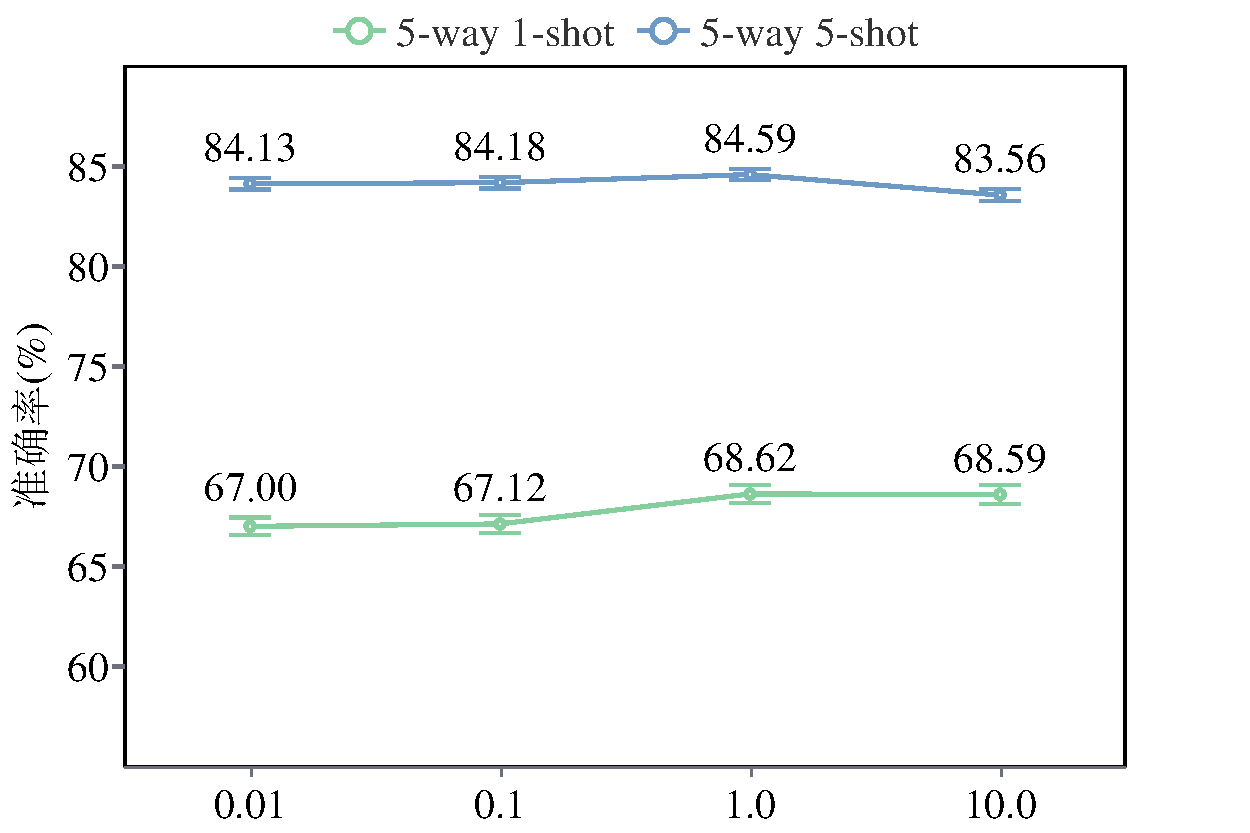
\includegraphics[width=\columnwidth]{figures/MGSRCL/miniImageNet/alpha.pdf}
\caption{$\alpha$}
\label{figure3: alpha(mini)}
\end{subfigure}
\begin{subfigure}{0.495\columnwidth}
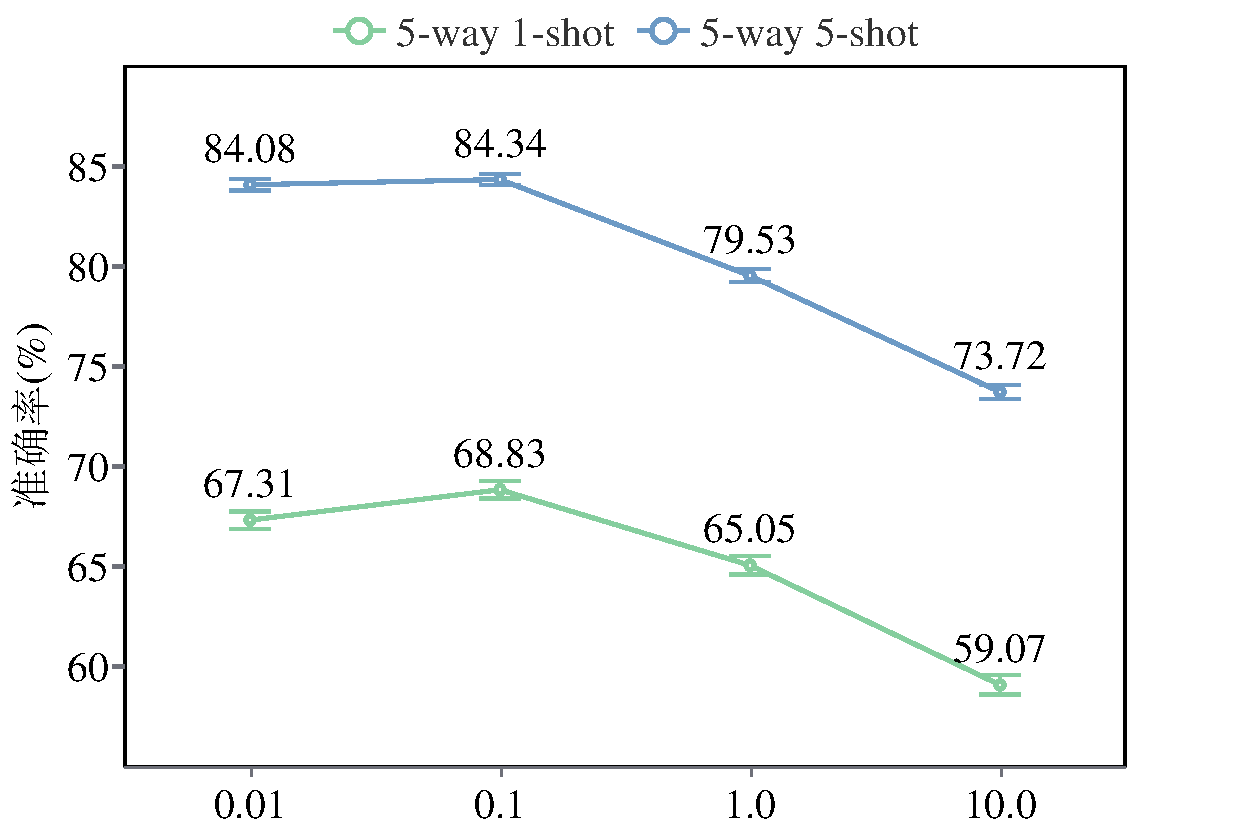
\includegraphics[width=\columnwidth]{figures/MGSRCL/miniImageNet/beta.pdf}
\caption{$\beta$}
\label{figure3: beta(mini)}
\end{subfigure}
\bicaption[MGSRCL在miniImageNet数据集上的超参数$\alpha$和$\beta$消融实验]{MGSRCL在miniImageNet数据集上的超参数$\alpha$和$\beta$消融实验。}[Hyperparameters $\alpha$ and $\beta$ ablation experiments of MGSRCL on miniImageNet]{Hyperparameters $\alpha$ and $\beta$ ablation experiments of MGSRCL on miniImageNet.}
\label{figure3: alpha and beta (mini)}
% \vspace{-4pt}
\end{figure}

\begin{figure}[h!]
\centering
\captionsetup{font={small, stretch=1.312}}
\begin{subfigure}{0.495\columnwidth}
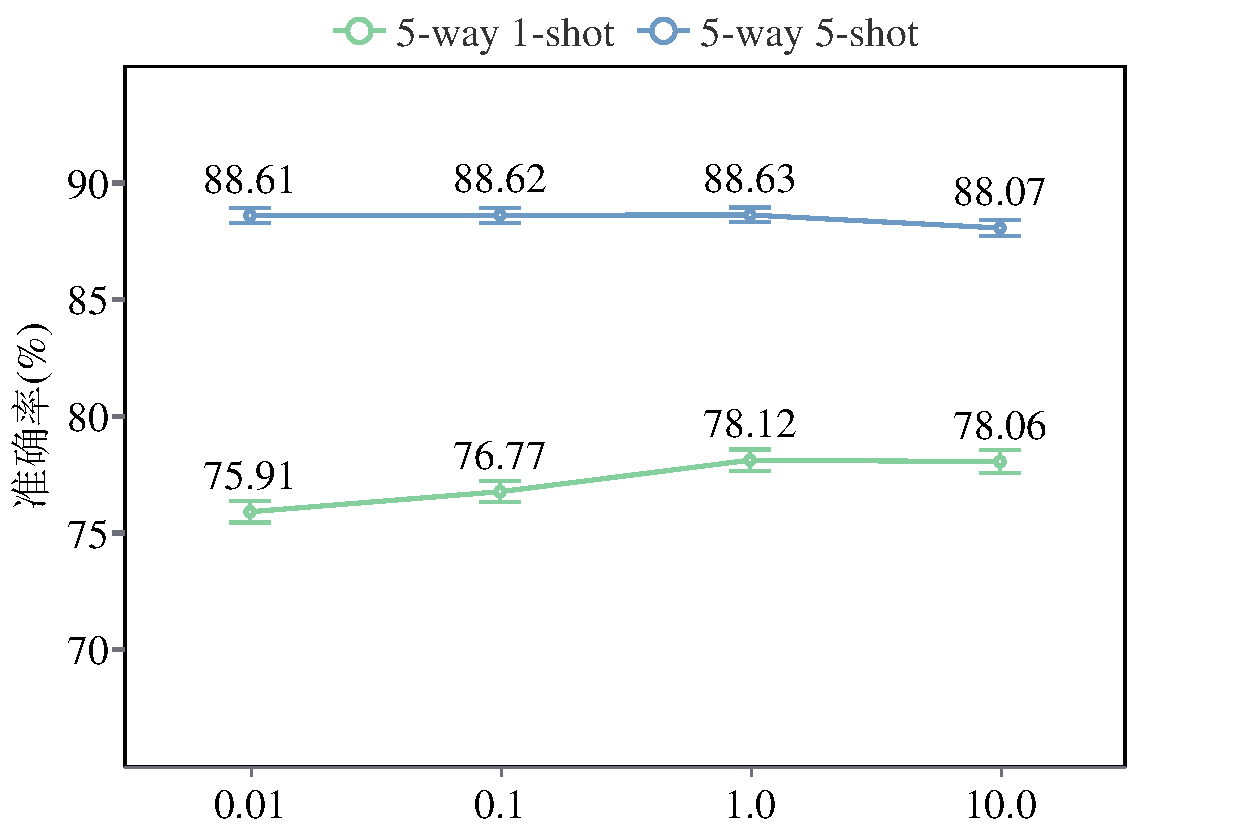
\includegraphics[width=\columnwidth]{figures/MGSRCL/CIFAR-FS/alpha.pdf}
\caption{$\alpha$}
\label{figure3: alpha(CIFAR-FS)}
\end{subfigure}
\begin{subfigure}{0.495\columnwidth}
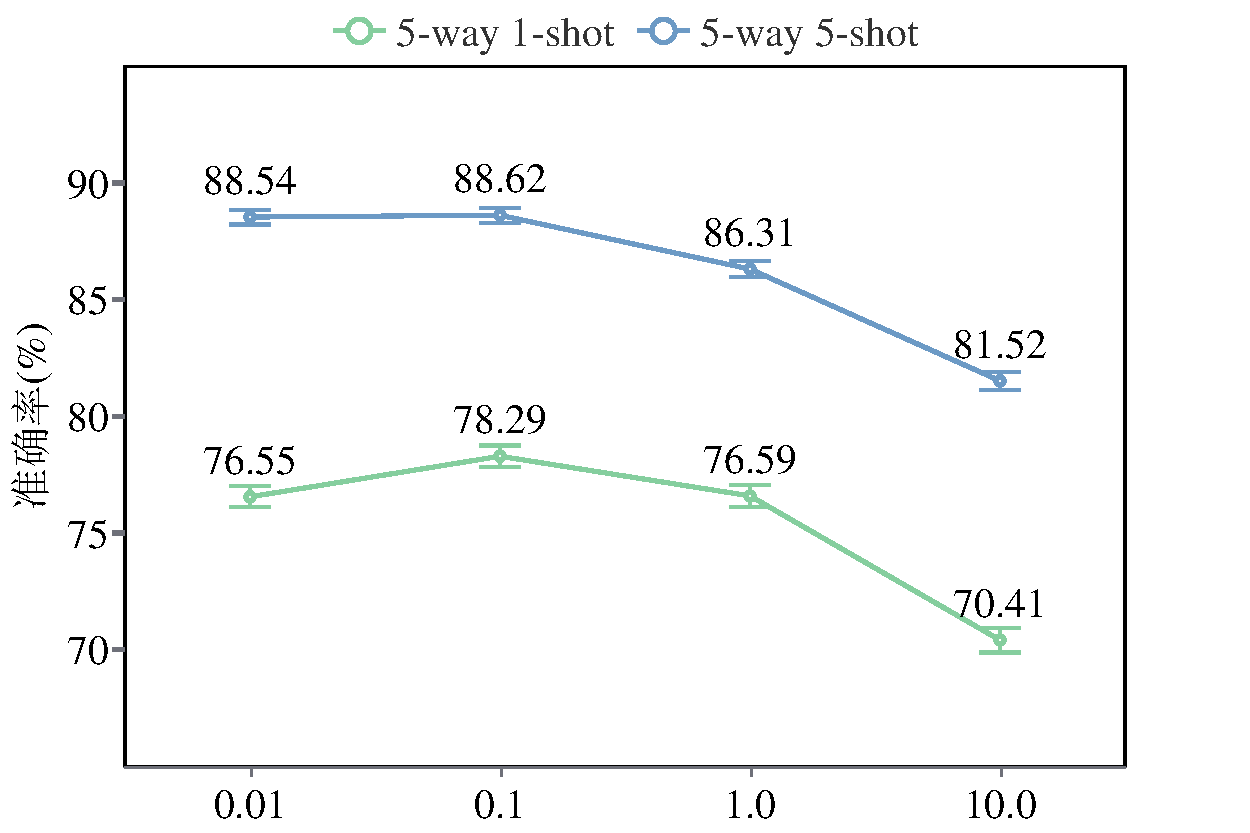
\includegraphics[width=\columnwidth]{figures/MGSRCL/CIFAR-FS/beta.pdf}
\caption{$\beta$}
\label{figure3: beta(CIFAR-FS)}
\end{subfigure}
\bicaption[MGSRCL在CIFAR-FS数据集上的超参数$\alpha$和$\beta$消融实验]{MGSRCL在CIFAR-FS数据集上的超参数$\alpha$和$\beta$消融实验。}[Hyperparameters $\alpha$ and $\beta$ ablation experiments of MGSRCL on CIFAR-FS]{Hyperparameters $\alpha$ and $\beta$ ablation experiments of MGSRCL on CIFAR-FS.}
\label{figure3: alpha and beta (CIFAR-FS)}
% \vspace{-5pt}
\end{figure}

\begin{figure}[h!]
\centering
\captionsetup{font={small, stretch=1.312}}
\begin{subfigure}{0.495\columnwidth}
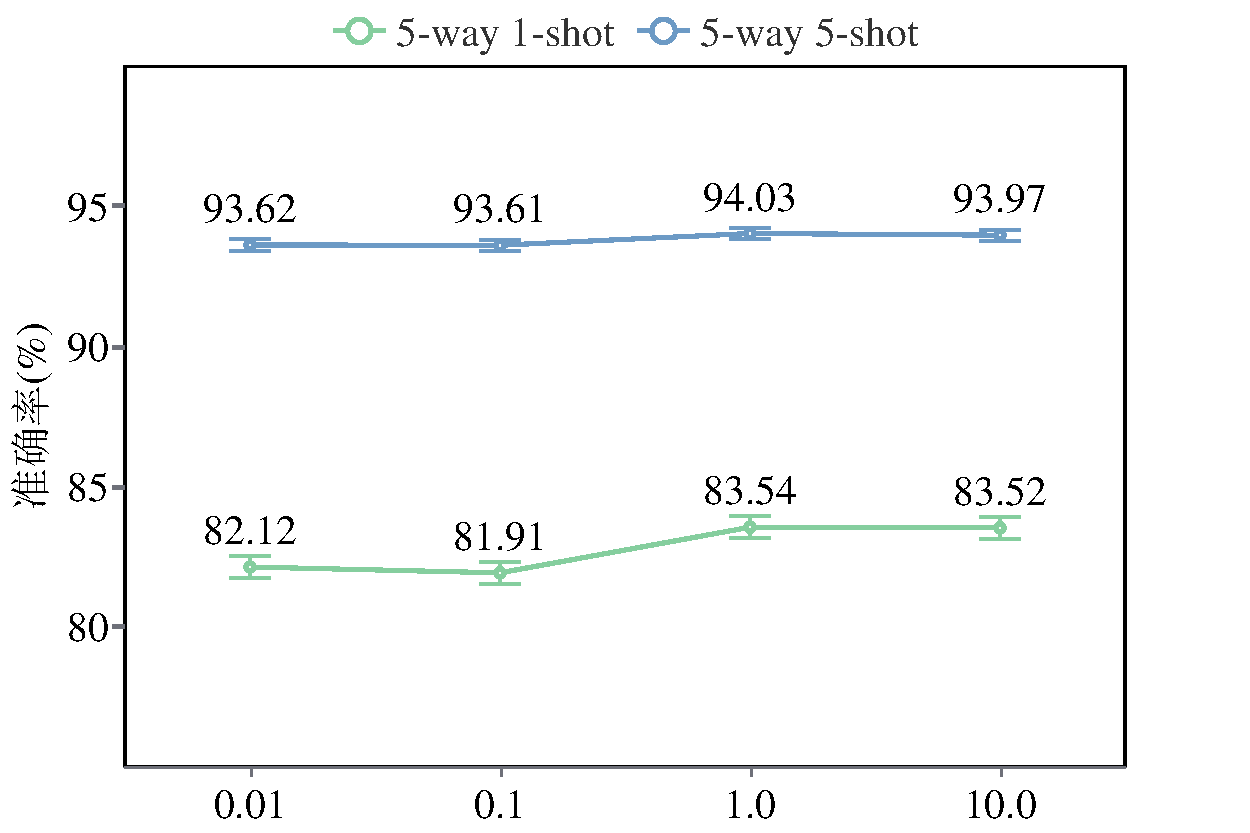
\includegraphics[width=\columnwidth]{figures/MGSRCL/CUB/alpha.pdf}
\caption{$\alpha$}
\label{figure3: alpha(CUB)}
\end{subfigure}
\begin{subfigure}{0.495\columnwidth}
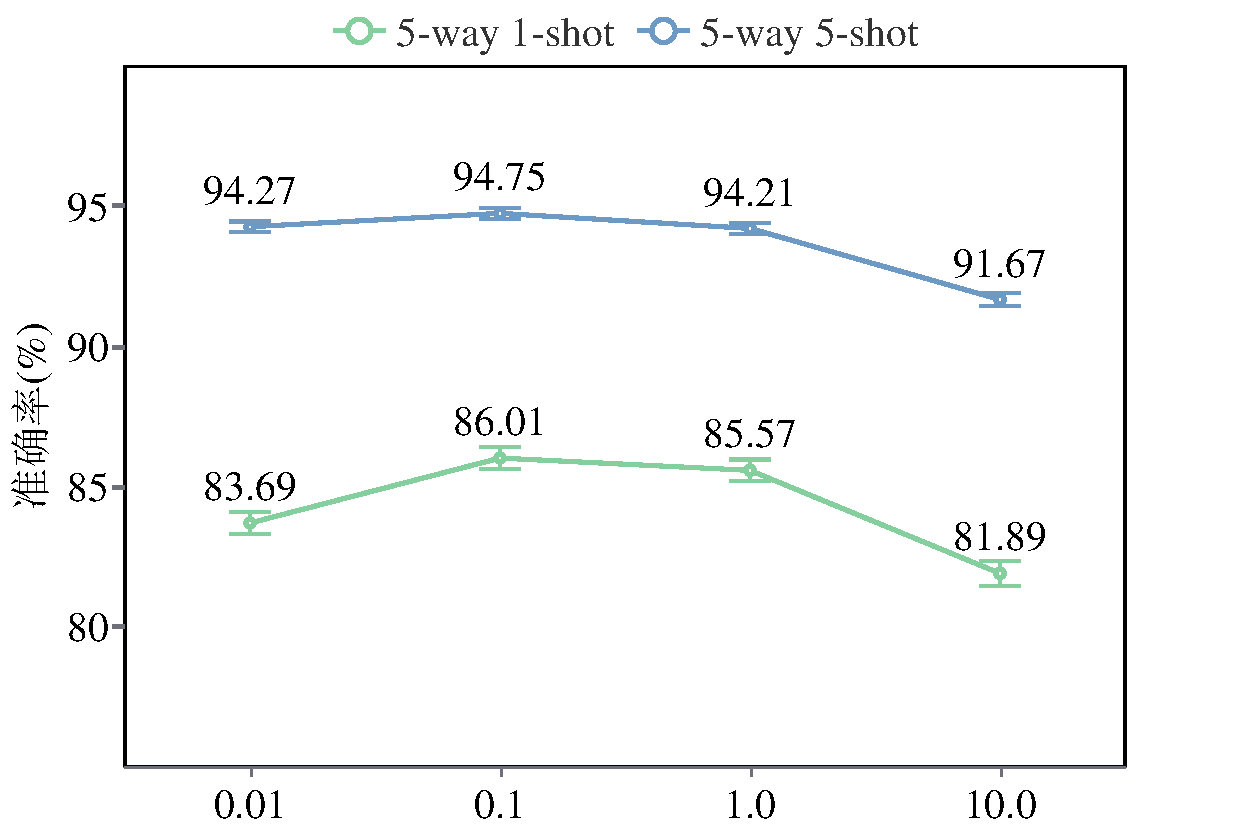
\includegraphics[width=\columnwidth]{figures/MGSRCL/CUB/beta.pdf}
\caption{$\beta$}
\label{figure3: beta(CUB)}
\end{subfigure}
\bicaption[MGSRCL在CUB数据集上的超参数$\alpha$和$\beta$消融实验]{MGSRCL在CUB数据集上的超参数$\alpha$和$\beta$消融实验。}[Hyperparameters $\alpha$ and $\beta$ ablation experiments of MGSRCL on CUB]{Hyperparameters $\alpha$ and $\beta$ ablation experiments of MGSRCL on CUB.}
\label{figure3: alpha and beta (CUB)}
% \vspace{-5pt}
\end{figure}

首先,为了观察模型分类结果随参数变化的趋势,在讨论一个超参数的影响时,本文将另一个超参数设置为0。如图\ref{figure3: alpha and beta (mini)}、\ref{figure3: alpha and beta (CIFAR-FS)}和\ref{figure3: alpha and beta (CUB)}所示,对于超参数$\alpha$,模型性能的变化较为平缓,整体呈现先上升再下降的趋势。当$\alpha = 1.0$时,模型性能在三个数据集上都达到最优,分别达到68.62\%、78.12\%和83.54\%的1-shot任务准确率以及84.59\%、88.63\%和94.03\%的5-shot准确率。而对于超参数$\beta$,随着$\beta$的增加,模型性能最初有所提高,然后呈现迅速下降的趋势,当$\beta = 0.1$时,模型性能达到最优,分别达到68.83\%、78.29\%和86.01\%的1-shot任务准确率以及84.34\%、88.62\%和94.75\%的5-shot任务准确率。


\begin{table}[h!]
\small    % 设置表格字体为5号
\setstretch{1.245}        % 设置具有指定弹力的橡皮长度(原行宽的1.2倍)
\captionsetup{font={small, stretch=1.512}}
\centering
% \vspace{-10pt}
\bicaption[MGSRCL在miniImageNet数据集上的超参数$\alpha$和$\beta$消融实验]{MGSRCL在miniImageNet数据集上的超参数$\alpha$和$\beta$消融实验。最优结果用粗体表示。}[Hyperparameters $\alpha$ and $\beta$ ablation experiments of MGSRCL on miniImageNet]{Hyperparameters $\alpha$ and $\beta$ ablation experiments of MGSRCL on miniImageNet. The best results are shown in bold.}
\begin{tabularx}{\textwidth}{lCCCC}
\toprule
\diagbox{${\alpha}$}{${\beta}$} & 0.01 & 0.1 & 1.0 & 10.0 \\
\midrule
0.01 & 67.57 $\pm$ 0.43 & 68.76 $\pm$ 0.44 & 65.71 $\pm$ 0.46 & 58.77 $\pm$ 0.47 \\
0.1 & 67.07 $\pm$ 0.43 & 68.82 $\pm$ 0.44 & 65.88 $\pm$ 0.46 & 59.53 $\pm$ 0.48 \\
1.0 & 68.95 $\pm$ 0.44 & \textbf{69.57 $\pm$ 0.45} & 66.68 $\pm$ 0.48 & 59.40 $\pm$ 0.48 \\
10.0 & 68.37 $\pm$ 0.46 & 69.22 $\pm$ 0.47 & 67.16 $\pm$ 0.48 & 59.25 $\pm$ 0.48 \\
\bottomrule
\end{tabularx}
\vspace{-15pt}
\label{table3: alpha and beta on miniImageNet}
\end{table}

\begin{table}[h!]
\small    % 设置表格字体为5号
\setstretch{1.245}        % 设置具有指定弹力的橡皮长度(原行宽的1.2倍)
\captionsetup{font={small, stretch=1.512}}
\centering
\bicaption[MGSRCL在CIFAR-FS数据集上的超参数$\alpha$和$\beta$消融实验]{MGSRCL在CIFAR-FS数据集上的超参数$\alpha$和$\beta$消融实验。最优结果用粗体表示。}[Hyperparameters $\alpha$ and $\beta$ ablation experiments of MGSRCL on CIFAR-FS]{Hyperparameters $\alpha$ and $\beta$ ablation experiments of MGSRCL on CIFAR-FS. The best results are shown in bold.}
\begin{tabularx}{\textwidth}{lCCCC}
\toprule
\diagbox{${\alpha}$}{${\beta}$} & 0.01 & 0.1 & 1.0 & 10.0 \\
\midrule
0.01 & 76.87 $\pm$ 0.46 & 78.06 $\pm$ 0.46 & 76.04 $\pm$ 0.49 & 71.23 $\pm$ 0.52 \\
0.1 & 77.12 $\pm$ 0.45 & 78.41 $\pm$ 0.46 & 76.67 $\pm$ 0.48 &  70.91 $\pm$ 0.53 \\
1.0 & 78.01 $\pm$ 0.47 & \textbf{78.54 $\pm$ 0.47} & 76.60 $\pm$ 0.50 & 70.45 $\pm$ 0.52 \\
10.0 & 78.02 $\pm$ 0.48 & 77.87 $\pm$ 0.49 & 76.46 $\pm$ 0.50 & 71.24 $\pm$ 0.52 \\
\bottomrule
\end{tabularx}
\vspace{-15pt}
\label{table3: alpha and beta on CIFAR-FS}
\end{table}

\begin{table}[h!]
\small    % 设置表格字体为5号
\setstretch{1.245}        % 设置具有指定弹力的橡皮长度(原行宽的1.2倍)
\captionsetup{font={small, stretch=1.512}}
\centering
\bicaption[MGSRCL在CUB数据集上的超参数$\alpha$和$\beta$消融实验]{MGSRCL在CUB数据集上的超参数$\alpha$和$\beta$消融实验。最优结果用粗体表示。}[Hyperparameters $\alpha$ and $\beta$ ablation experiments of MGSRCL on CUB]{Hyperparameters $\alpha$ and $\beta$ ablation experiments of MGSRCL on CUB. The best results are shown in bold.}
\begin{tabularx}{\textwidth}{lCCCC}
\toprule
\diagbox{${\alpha}$}{${\beta}$} & 0.01 & 0.1 & 1.0 & 10.0 \\
\midrule
0.01 & 82.79 $\pm$ 0.39 & 86.00 $\pm$ 0.38 & 85.42 $\pm$ 0.38 & 82.24 $\pm$ 0.43 \\
0.1 & 82.89 $\pm$ 0.39 & 85.86 $\pm$ 0.37 & 86.07 $\pm$ 0.37 & 81.83 $\pm$ 0.44 \\
1.0 & 83.82 $\pm$ 0.39 & \textbf{86.14 $\pm$ 0.38} & 86.09 $\pm$ 0.38 & 81.87 $\pm$ 0.44 \\
10.0 & 85.12 $\pm$ 0.39 & 85.81 $\pm$ 0.38 & 86.07 $\pm$ 0.39 & 80.63 $\pm$ 0.46 \\
\bottomrule
\end{tabularx}
% \vspace{-15pt}
\label{table3: alpha and beta on CUB}
\end{table}

另外,为了全面准确地确定超参数${\alpha}$和${\beta}$的最优值,本文采用网格搜索调参法来进行实验,在miniImageNet、CIFAR-FS和CUB数据集上5-way 1-shot少样本分类任务的实验结果分别如表\ref{table3: alpha and beta on miniImageNet}、\ref{table3: alpha and beta on CIFAR-FS}和\ref{table3: alpha and beta on CUB}所示。实验结果表明,当${\alpha}$和${\beta}$分别设置为1.0和0.1时,模型在三个数据集上同时达到最优性能,1-shot任务准确率分别为69.57\%、78.54\%和86.14\%。因此,在最终模型中,本文将$\alpha$设置为1.0,$\beta$设置为0.1。


\begin{figure}[h!]
\centering
\captionsetup{font={small, stretch=1.312}}
\begin{subfigure}{0.495\columnwidth}
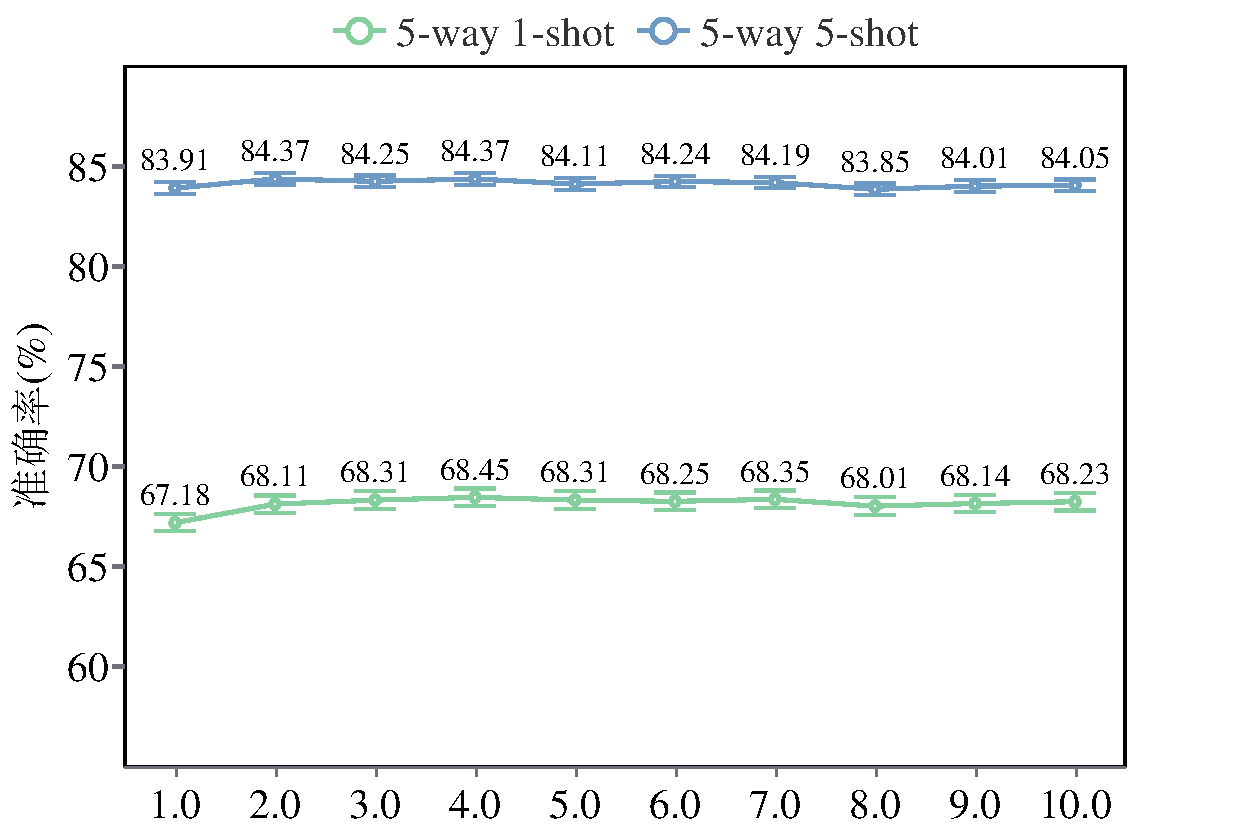
\includegraphics[width=\columnwidth]{figures/MGSRCL/miniImageNet/t1.pdf}
\caption{$\tau_1$}
\label{figure3: t1(mini)}
\end{subfigure}
\begin{subfigure}{0.495\columnwidth}
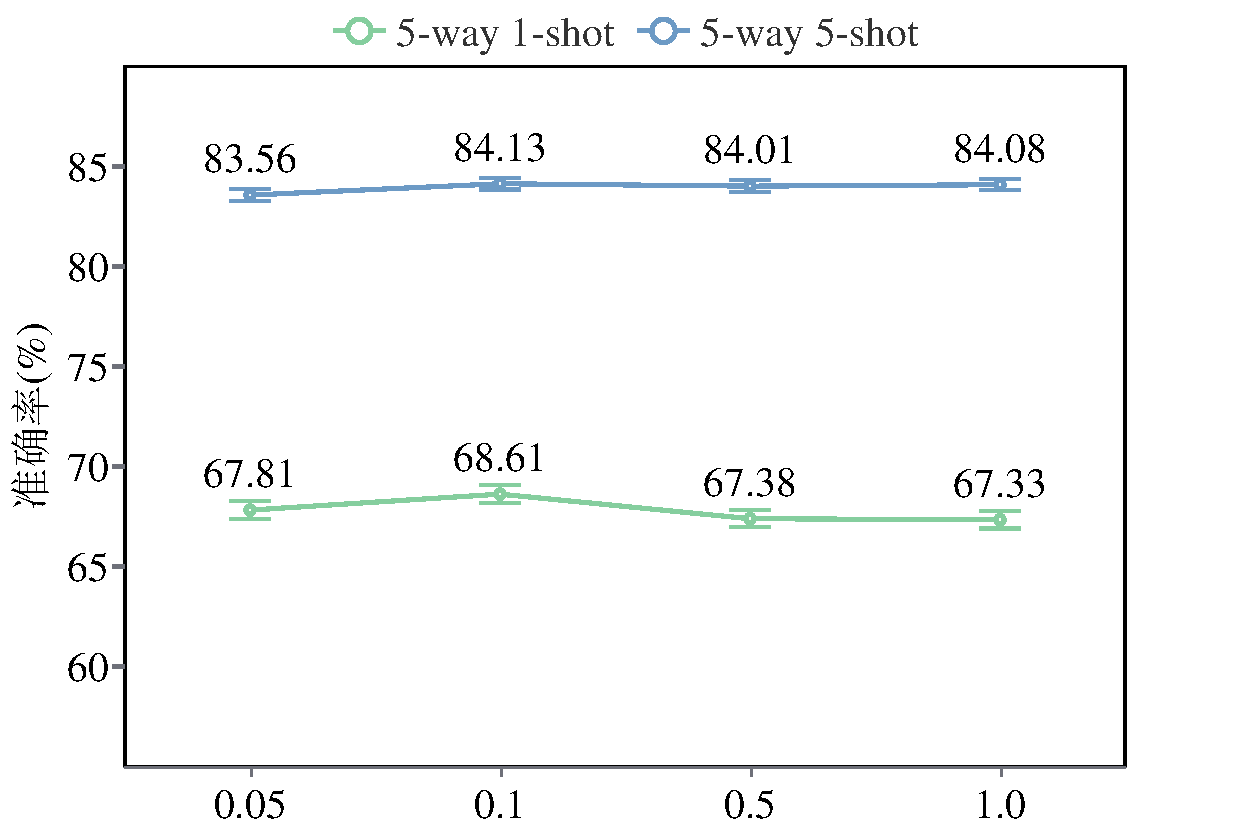
\includegraphics[width=\columnwidth]{figures/MGSRCL/miniImageNet/t2.pdf}
\caption{$\tau_2$}
\label{figure3: t2(mini)}
\end{subfigure}
\bicaption[MGSRCL在miniImageNet数据集上的超参数$\tau_1$和$\tau_2$消融实验]{MGSRCL在miniImageNet数据集上的超参数$\tau_1$和$\tau_2$消融实验。}[Hyperparameters $\tau_1$ and $\tau_2$ ablation experiments of MGSRCL on miniImageNet]{Hyperparameters $\tau_1$ and $\tau_2$ ablation experiments of MGSRCL on miniImageNet.}
\label{figure3: t1 and t2 (mini)}
% \vspace{-10pt}
\end{figure}

\begin{figure}[h!]
\centering
\captionsetup{font={small, stretch=1.312}}
\begin{subfigure}{0.495\columnwidth}
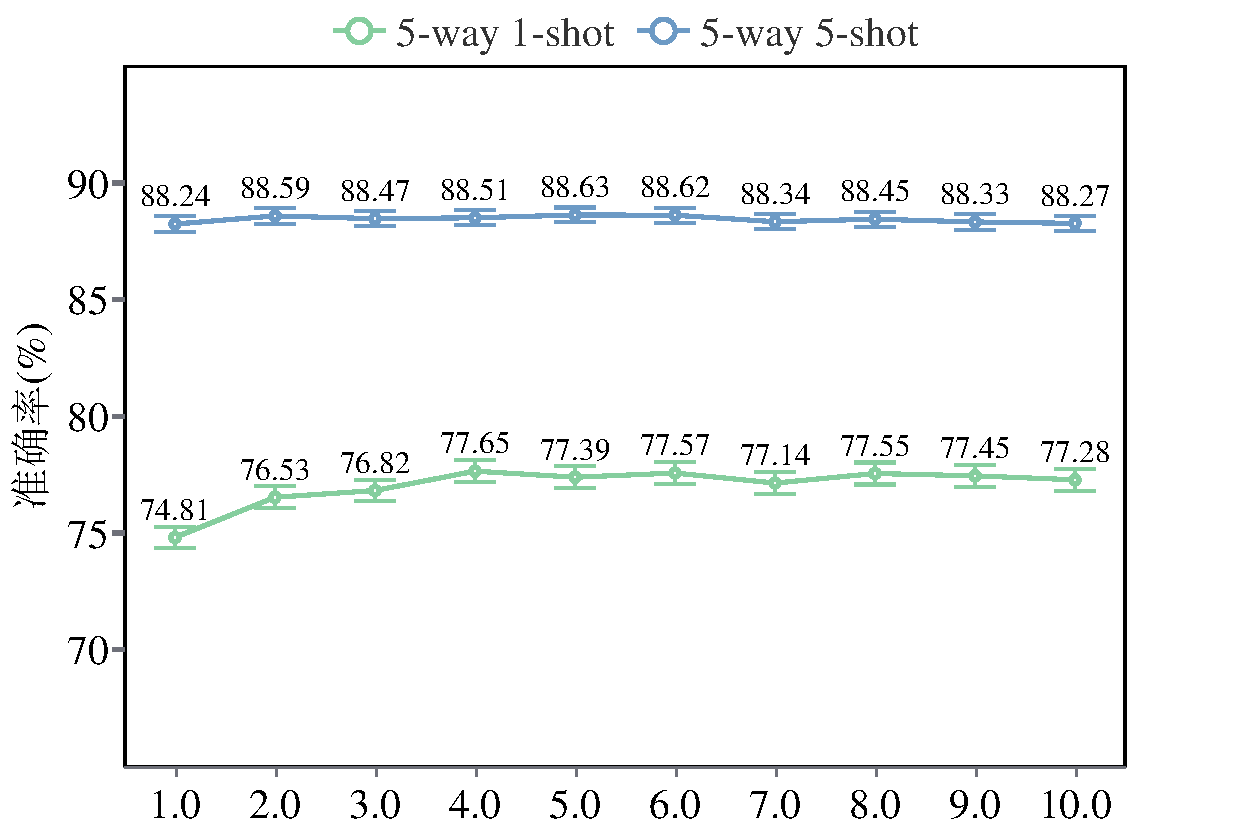
\includegraphics[width=\columnwidth]{figures/MGSRCL/CIFAR-FS/t1.pdf}
\caption{$\tau_1$}
\label{figure3: t1(CIFAR-FS)}
\end{subfigure}
\begin{subfigure}{0.495\columnwidth}
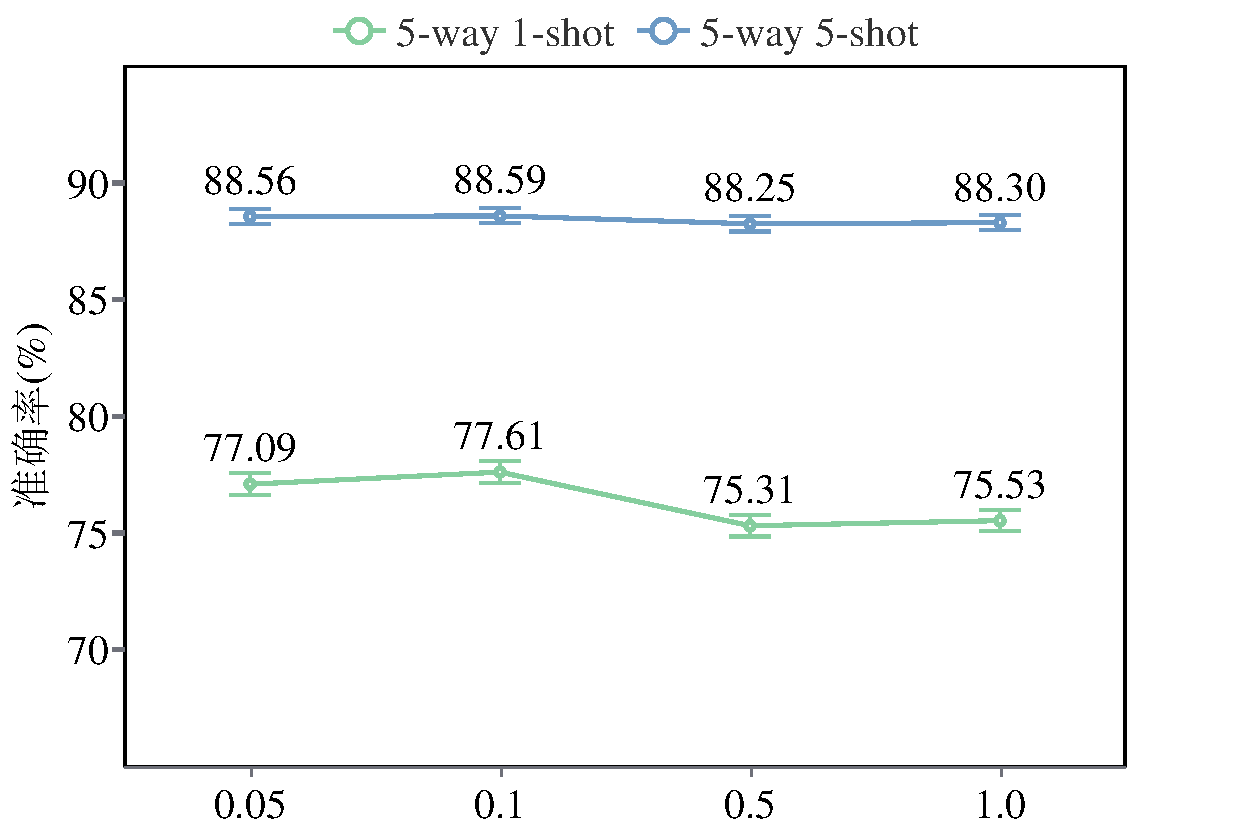
\includegraphics[width=\columnwidth]{figures/MGSRCL/CIFAR-FS/t2.pdf}
\caption{$\tau_2$}
\label{figure3: t2(CIFAR-FS)}
\end{subfigure}
\bicaption[MGSRCL在CIFAR-FS数据集上的超参数$\tau_1$和$\tau_2$消融实验]{MGSRCL在CIFAR-FS数据集上的超参数$\tau_1$和$\tau_2$消融实验。}[Hyperparameters $\tau_1$ and $\tau_2$ ablation experiments of MGSRCL on CIFAR-FS]{Hyperparameters $\tau_1$ and $\tau_2$ ablation experiments of MGSRCL on CIFAR-FS.}
\label{figure3: t1 and t2 (CIFAR-FS)}
% \vspace{-7pt}
\end{figure}

\begin{figure}[h!]
\centering
\captionsetup{font={small, stretch=1.312}}
\begin{subfigure}{0.495\columnwidth}
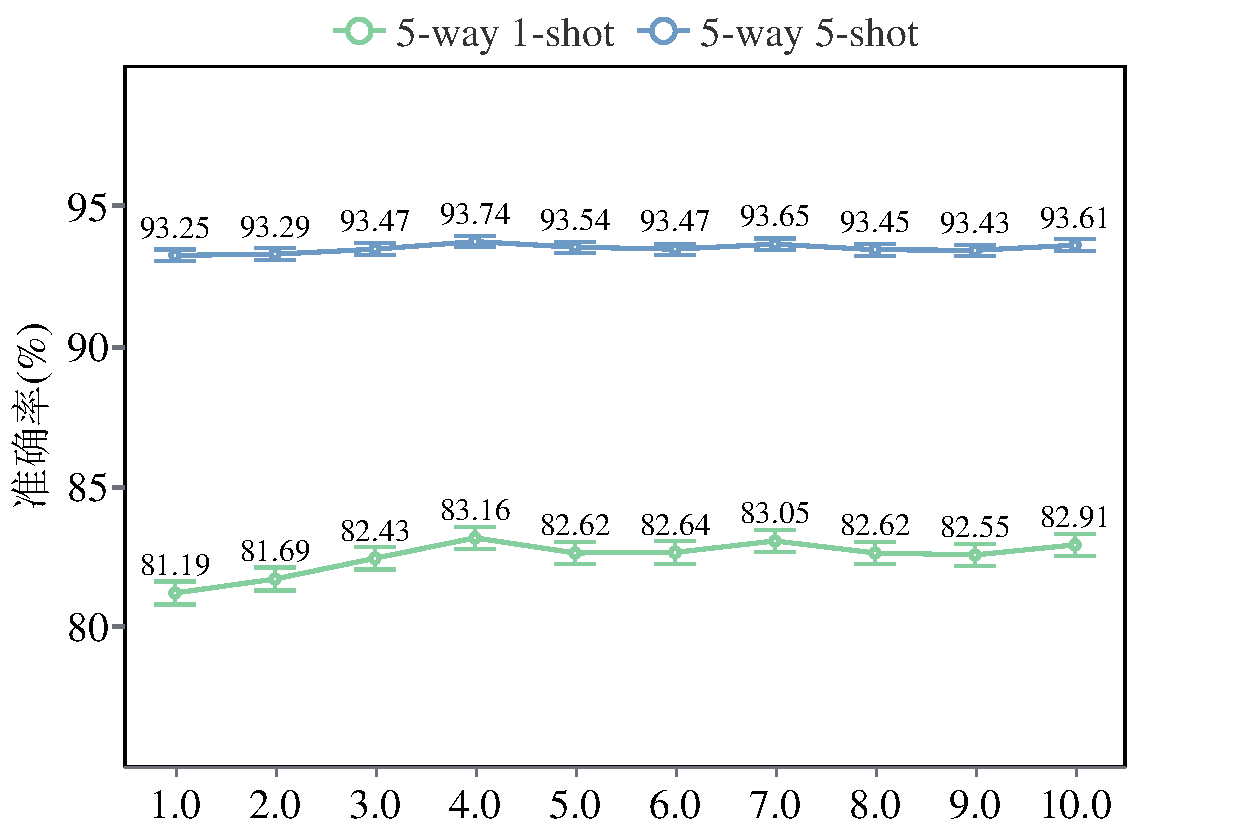
\includegraphics[width=\columnwidth]{figures/MGSRCL/CUB/t1.pdf}
\caption{$\tau_1$}
\label{figure3: t1(CUB)}
\end{subfigure}
\begin{subfigure}{0.495\columnwidth}
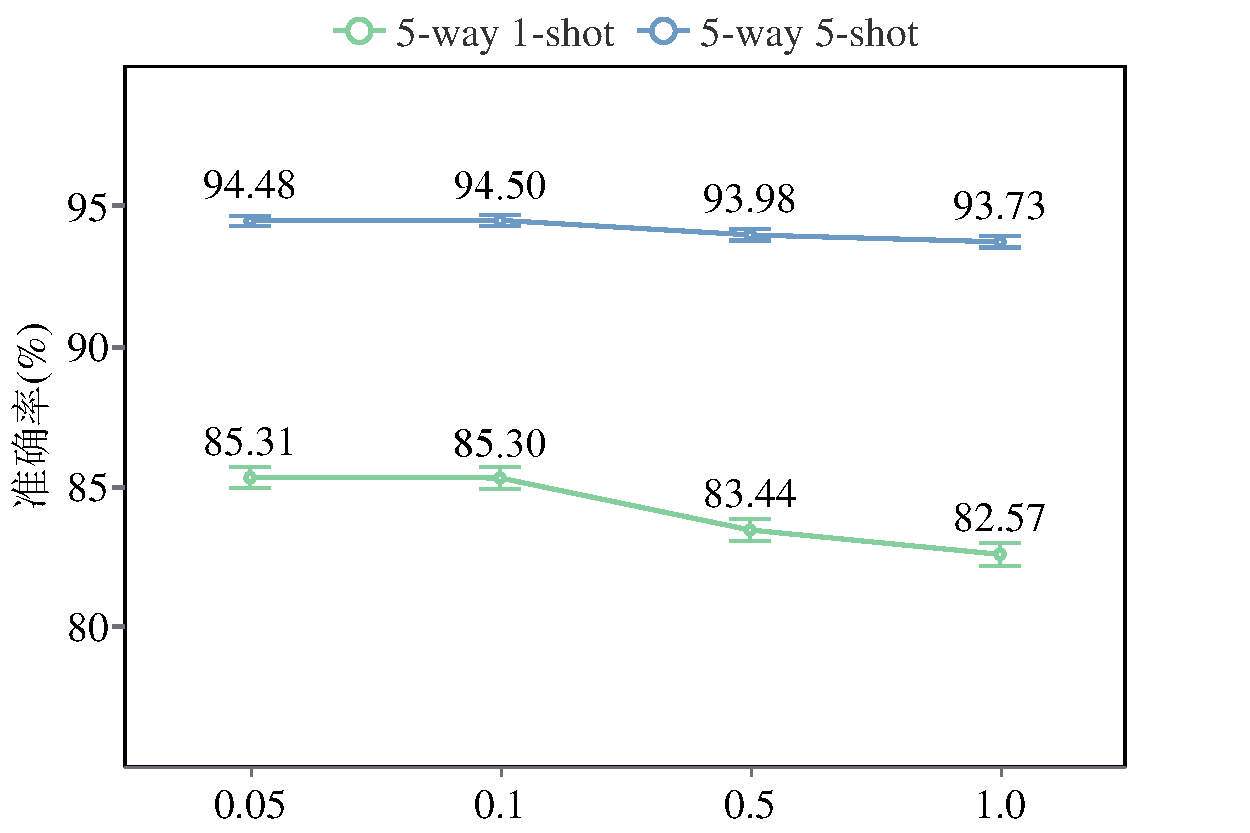
\includegraphics[width=\columnwidth]{figures/MGSRCL/CUB/t2.pdf}
\caption{$\tau_2$}
\label{figure3: t2(CUB)}
\end{subfigure}
\bicaption[MGSRCL在CUB数据集上的超参数$\tau_1$和$\tau_2$消融实验]{MGSRCL在CUB数据集上的超参数$\tau_1$和$\tau_2$消融实验。}[Hyperparameters $\tau_1$ and $\tau_2$ ablation experiments of MGSRCL on CUB]{Hyperparameters $\tau_1$ and $\tau_2$ ablation experiments of MGSRCL on CUB.}
\label{figure3: t1 and t2 (CUB)}
% \vspace{-7pt}
\end{figure}

\textbf{(3)讨论超参数$\tau_1$和$\tau_2$对模型性能的影响}

此外,本文还讨论了温度参数$\tau_1$和$\tau_2$对实验结果的影响。为了更清晰地观察温度参数在对应模块中起到的作用,在讨论温度参数时,本文只保留了相关模块,去除了其他模块。首先,$\tau_1$用于平滑预测输出以提供更多概率分布差异信息,本文令其从1.0到10.0变化,在miniImageNet、CIFAR-FS和CUB三个数据集上评估模型分类性能。如图\ref{figure3: t1 and t2 (mini)}、\ref{figure3: t1 and t2 (CIFAR-FS)}和\ref{figure3: t1 and t2 (CUB)}所示,当$\tau_1$从1.0变化到10.0时,实验结果并未发生显著变化。当执行5-way 1-shot分类任务时,三个数据集都在$\tau_1$设置为4.0时取得了最优结果,执行5-way 5-shot分类任务时,miniImageNet和CUB数据集的也都在$\tau_1$设置为4.0时取得了最优结果,CIFAR-FS则是在$\tau_1$设置为5.0时取得了最优结果。综合考虑,最终将$\tau_1$设置为4.0。$\tau_2$是CCL组件中使用的温度参数。本文评估了当$\tau_2$设置为0.05、0.1、0.5和1.0时的模型性能。除了在CUB数据集的5-way 1-shot分类任务上将$\tau_2$设置为0.05时取得了最优结果,其余数据集以及5-way 5-shot任务均是当$\tau_2 = 0.1$时模型达到了最优结果。因此,在最终模型中,MGSRCL将$\tau_2$设置为0.1。


\begin{figure}[h!]
  \centering
  \captionsetup{font={small, stretch=1.312}}
  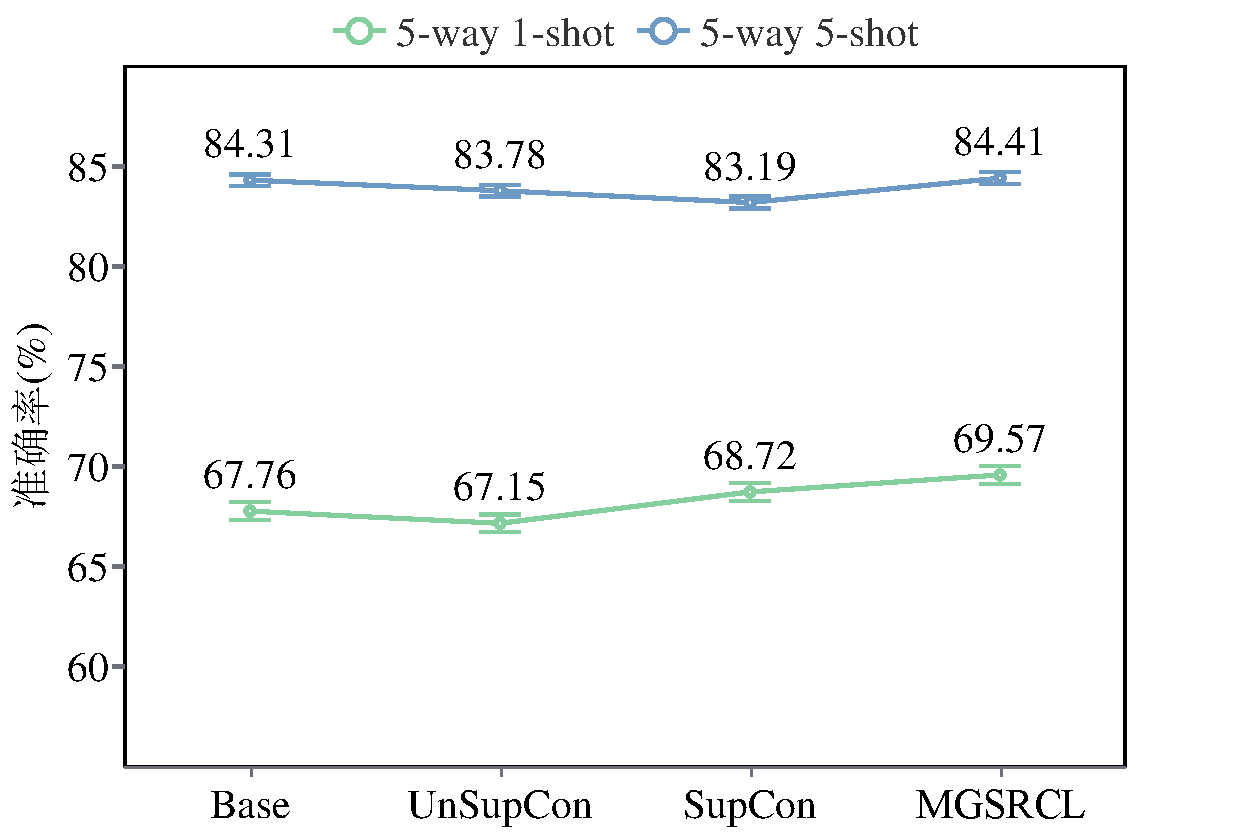
\includegraphics[width=0.6\columnwidth]{figures/MGSRCL/miniImageNet/comparison.pdf}
  \bicaption[在miniImageNet数据集上的不同样本关系挖掘策略对比实验]{在miniImageNet数据集上的不同样本关系挖掘策略对比实验。}[Experimental comparison of different sample relationship mining strategies on miniImageNet]{Experimental comparison of different sample relationship mining strategies on miniImageNet.}
  \label{figure3: comparison(miniImageNet)}
\end{figure}

\begin{figure}[h!]
  \centering
  \captionsetup{font={small, stretch=1.312}}
  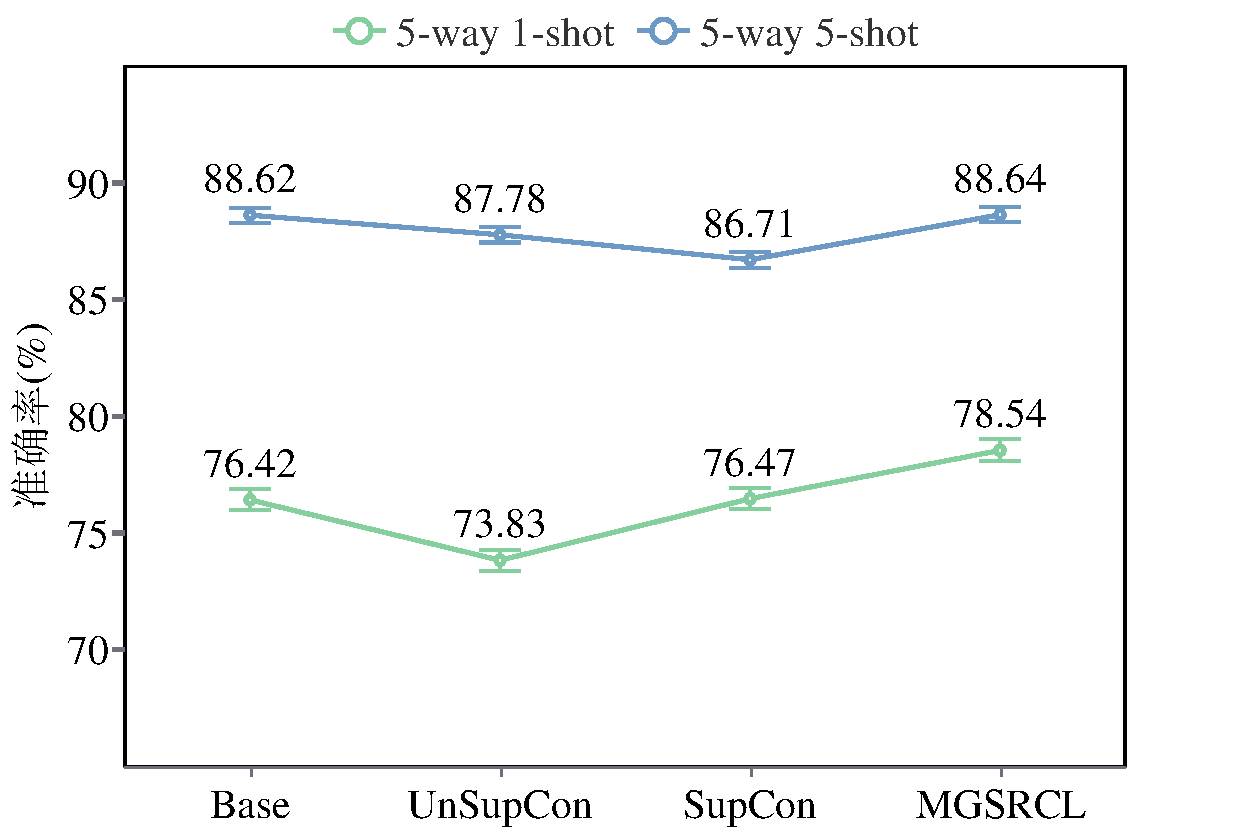
\includegraphics[width=0.6\columnwidth]{figures/MGSRCL/CIFAR-FS/comparison.pdf}
  \bicaption[在CIFAR-FS数据集上的不同样本关系挖掘策略对比实验]{在CIFAR-FS数据集上的不同样本关系挖掘策略对比实验。}[Experimental comparison of different sample relationship mining strategies on CIFAR-FS]{Experimental comparison of different sample relationship mining strategies on CIFAR-FS.}
  \label{figure3: comparison(CIFAR-FS)}
\end{figure}

\begin{figure}[h!]
  \centering
  \captionsetup{font={small, stretch=1.312}}
  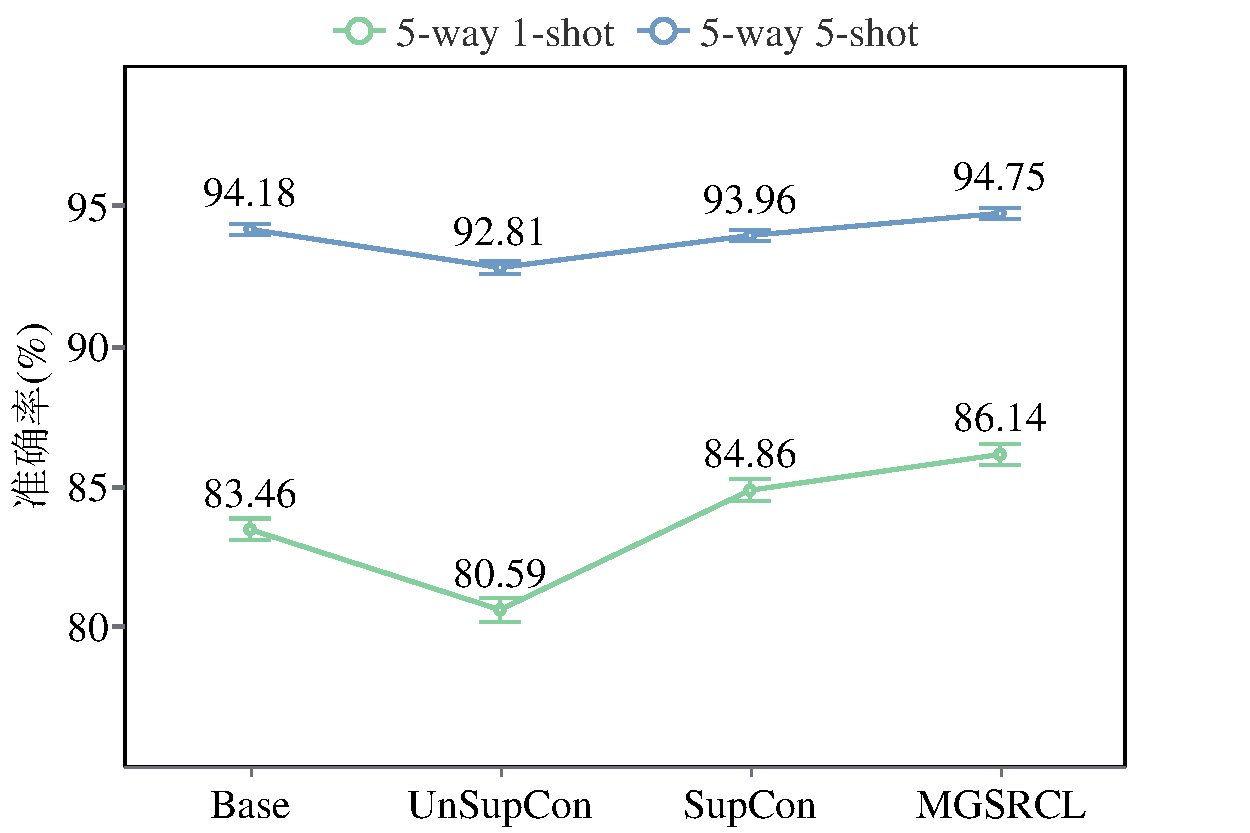
\includegraphics[width=0.6\columnwidth]{figures/MGSRCL/CUB/comparison.pdf}
  \bicaption[在CUB数据集上的不同样本关系挖掘策略对比实验]{在CUB数据集上的不同样本关系挖掘策略对比实验。}[Experimental comparison of different sample relationship mining strategies on CUB]{Experimental comparison of different sample relationship mining strategies on CUB.}
  \label{figure3: comparison(CUB)}
\end{figure}

\textbf{(4)样本关系挖掘策略探讨}

近年来,一些少样本分类方法利用对比学习来挖掘样本关系。然而,这些方法通常直接使用无监督对比学习(Unsupervised Contrastive Learning,简称UnSupCon)\cite{SimCLR}或有监督对比学习(Supervised Contrastive Learning,简称SupCon)\cite{SupCon}作为辅助损失,这使得它们未能充分挖掘样本间的关系。为了表明本文方法相较于这些方法的优越性,本文基于所提出的基础特征学习网络进行了实验\footnote{此处,本文使用了SupCon提供的代码来实现无监督对比学习方法(SimCLR)和有监督对比学习方法(SupCon)。源代码可在\href{https://github.com/HobbitLong/SupContrast}{https://github.com/HobbitLong/SupContrast}获取。}。在实施过程中,UnSupCon和SupCon损失作为辅助损失被直接添加到原基础特征学习网络中,与本文方法相同。如图\ref{figure3: comparison(miniImageNet)}、\ref{figure3: comparison(CIFAR-FS)}和\ref{figure3: comparison(CUB)}所示,在miniImageNet、CIFAR-FS和CUB数据集上,添加UnSupCon后模型性能无论是1-shot分类任务还是5-shot分类任务,结果与基础模型相比都有所下降。这可以归因于UnSupCon将图像的变换视为正样本,而将其他图像视为负样本,会导致其在特征空间将同类样本推远,从而造成性能下降。另一方面,将SupCon整合到模型中并未受到此问题的影响,虽然在5-way 5-shot少样本分类任务上结果略微降低,但其在1-shot分类任务上结果都有所提升,且在miniImageNet与CUB数据集上提升明显。然而,SupCon将一个样本的变换及其同类样本视为相同的关系,这是不合适的,因为一个样本的不同变换应具有一致的语义内容,而同类样本的语义内容应仅相似而不是完全一致。相比之下,本文提出的方法充分考虑了不同粒度的样本关系,并对它们进行了细致地建模,从而在三个数据集上都取得了最优结果,这表明了本文方法更充分地挖掘了样本关系并对其进行了有效建模。


\begin{figure}[h!]
    \centering
    \captionsetup{font={small, stretch=1.312}}
    \begin{subfigure}{0.24\columnwidth}
    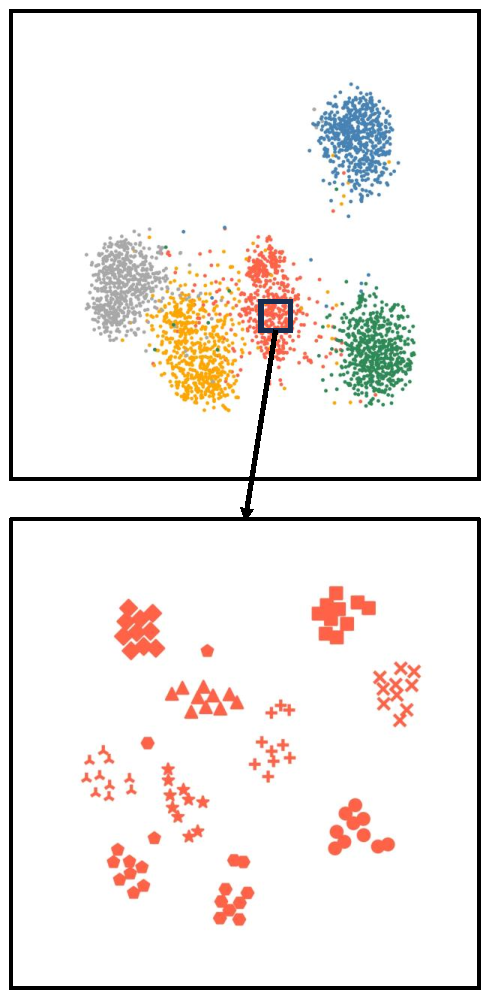
\includegraphics[width=\columnwidth]{figures/MGSRCL/t-SNE/Base.pdf}
    \caption{Base}
    \label{figure3: t-SNE Base}
    \end{subfigure}
    \begin{subfigure}{0.24\columnwidth}
    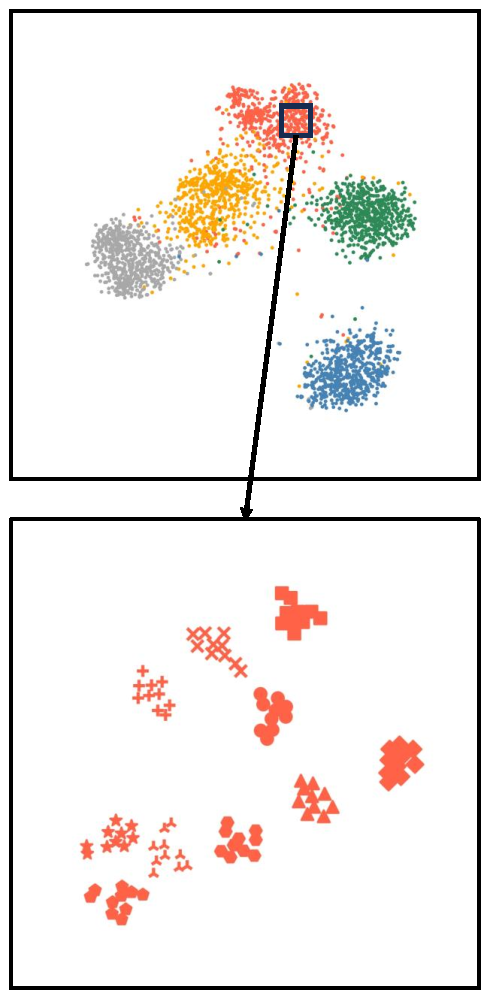
\includegraphics[width=\columnwidth]{figures/MGSRCL/t-SNE/Base + TCL.pdf}
    \caption{Base + TCL}
    \label{figure3: t-SNE Base + TCL}
    \end{subfigure}
    \begin{subfigure}{0.24\columnwidth}
    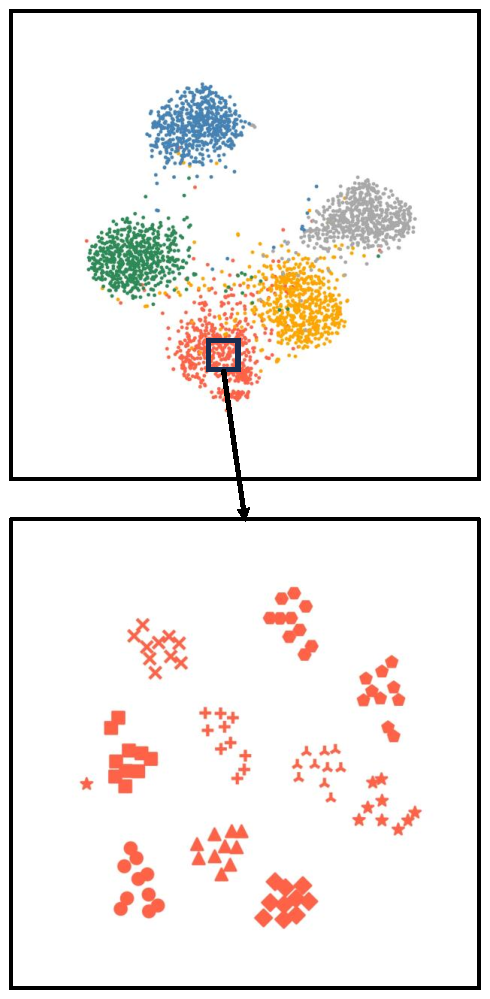
\includegraphics[width=\columnwidth]{figures/MGSRCL/t-SNE/Base + CCL.pdf}
    \caption{Base + CCL}
    \label{figure3: t-SNE Base + CCL}
    \end{subfigure}
    \begin{subfigure}{0.24\columnwidth}
    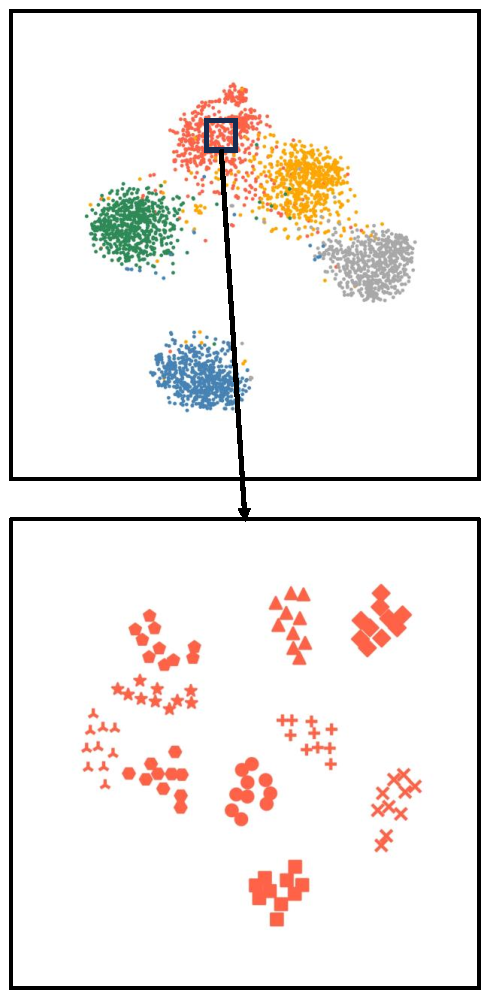
\includegraphics[width=\columnwidth]{figures/MGSRCL/t-SNE/Ours.pdf}
    \caption{MGSRCL}
    \label{figure3: t-SNE MGSRCL}
    \end{subfigure}
    \bicaption[miniImageNet数据集上不同模型所提取特征的t-SNE可视化结果]{miniImageNet数据集上不同模型所提取特征的t-SNE可视化结果。不同颜色代表不同类别(第一行),同一形状代表同一样本的不同变换版本(第二行)。}[The t-SNE visualization results of features extracted by different models on miniImageNet]{The t-SNE visualization results of features extracted by different models on miniImageNet. Different colors represent different categories (first row), and the same shape represents different transformed versions of the same sample (second row).}
    \label{figure3: t-SNE}
\end{figure}


\subsection[\hspace{-2pt}可视化分析]{{\heiti\zihao{4} \hspace{-8pt}可视化分析}}\label{section3: 可视化分析}

为了更好地展示MGSRCL模型的有效性,本文在miniImageNet上随机选取了5个新类,并使用t-SNE对不同模型提取的特征进行了可视化实验,如图\ref{figure3: t-SNE}所示,其中Base表示本文的基础特征学习网络,Base + TCL和Base + CCL分别代表基础特征学习网络整合了TCL模块以及CCL模块,而MGSRCL则代表本文的最终模型。在此图里,第一行展示了类内样本关系和类间样本关系,第二行则是展示了样本内关系,其中第一行图用不同颜色代表不同的类,第二行图则是将同一样本的不同变换版本用同一个形状表示。为便于检验第一行分类边界的质量,本文提供了如下数值数据:$d_1/d_2$,其中$d_1$表示五个类别样本与其样本中心间平均距离的均值(即类内样本内聚度),$d_2$则表征各类别中心之间距离的平均值(即不同类别中心间的离散度)。具体数值如下:(a) Base:1.01,(b) Base + TCL:0.99,(c) Base + CCL:0.91,(d) MGSRCL:0.90。这些数据直观地反映了不同模型在分类边界质量上的表现差异。首先,在第一行图中,可以观察到基础特征学习网络模型Base已经具有明确的分类边界,如图\ref{figure3: t-SNE Base}所示,这证明使用全部基类数据训练一个特征提取网络便可取得一个较好的效果。与Base模型和Base + TCL模型相比,在Base + CCL模型和最终的MGSRCL模型中,同一类别内的样本表现出更好的内聚性,不同类样本之间边界更加明显,这证明了约束同类样本的类内关系和不同类样本的类间关系的有效性。此外,通过约束同一样本在不同变换下的样本内关系,同一样本不同变换版本可以在特征空间保持更好的一致性,如图\ref{figure3: t-SNE Base + TCL}和图\ref{figure3: t-SNE MGSRCL}中的第二行图所示。而在其他模型中,一些变换的特征与其他变换的特征相距甚远,这展示了TCL模块的作用。综上所述,通过可视化实验证明,本文所提方法通过约束多种粒度的样本关系,对不同的样本关系进行了细致有效的建模,使得模型在新类上所提取的特征具有更好的判别性,从而达到了更高的分类准确率。

\section[\hspace{-2pt}本章小结]{{\heiti\zihao{-3} \hspace{-8pt}本章小结}}\label{section3: 本章小结}

本章研究基于多粒度样本关系建模的少样本特征学习算法,针对少样本特征学习模型由于基类数据和新类数据类别不同而面临的模型特征提取能力不足的问题,充分挖掘了多种粒度的样本关系,并通过对比学习对多粒度样本关系进行建模,提出了一种多粒度样本关系对比学习(Multi-Grained Sample Relation Contrastive Learning,简称MGSRCL)方法,以帮助模型提取到更具判别性的样本特征。MGSRCL方法使用一致性学习(TCL)模块通过标签分布对齐约束同一样本的不同变换具有一致的语义内容从而对样本内关系进行建模,以及类对比学习(CCL)模块通过拉近同类样本特征,同时推远不同类样本特征从而对类内样本关系以及类间样本关系进行建模。此外,还利用自监督学习技术令网络学习图像进行了何种变换,来增强基础特征学习网络的特征学习能力。在miniImageNet、tieredImageNet、CIFAR-FS和CUB-200-2011数据集的大量实验表明,MGSRCL在各个少样本基准数据集都取得了优异的性能表现,并且还可以作为预训练模型整合到其他两阶段少样本分类方法中提升它们的分类性能。

综上所述,本章提出的基于多粒度样本关系建模的少样本特征学习算法通过对多种样本关系进行建模,充分挖掘了不同样本间的关系信息,提高了网络所提取特征的质量,并可以为其他少样本分类算法提供优质的预训练网络和高质量的样本特征。

